\documentclass[11pt]{article}
\usepackage[textwidth=18.0cm, textheight=23.0cm, top=2.0cm]{geometry}
\usepackage{pst-all}
\usepackage{amssymb}
\usepackage{tikz}
\usepackage{underscore}\begin{document}
\pagestyle{empty}


ClassName: \underline{\textbf{Class_03.2bp-41}}
\par
BinSize: \underline{\textbf{40 × 40}}
\par
ReduceSize: \underline{\textbf{40 × 40}}
\par
TypeNum: \underline{\textbf{96}}
\par
Num: \underline{\textbf{100}}
\par
OutS: \underline{\textbf{35200}}
\par
InS: \underline{\textbf{33240}}
\par
Rate: \underline{\textbf{0.944}}
\par
UB: \underline{\textbf{22}}
\par
LB0: \underline{\textbf{22}}
\par
LB: \underline{\textbf{22}}
\par
LBWithCut: \underline{\textbf{22}}
\par
NodeCut: \underline{\textbf{0}}
\par
ExtendedNodeCnt: \underline{\textbf{1}}
\par
GenNodeCnt: \underline{\textbf{1}}
\par
PrimalNode: \underline{\textbf{0}}
\par
ColumnCount: \underline{\textbf{22}}
\par
TotalCutCount: \underline{\textbf{0}}
\par
RootCutCount: \underline{\textbf{0}}
\par
LPSolverCnt: \underline{\textbf{1}}
\par
PricingSolverCnt: \underline{\textbf{0}}
\par
BranchAndBoundNum: \underline{\textbf{1}}
\par
isOpt: \underline{\textbf{true}}
\par
TimeOnInitSolution: \underline{\textbf{600.000 s}}
\par
TimeOnPrimal: \underline{\textbf{0.000 s}}
\par
TimeOnPricing: \underline{\textbf{0.000 s}}
\par
TimeOnRmp: \underline{\textbf{0.078 s}}
\par
TotalTime: \underline{\textbf{600.359 s}}
\par
\newpage


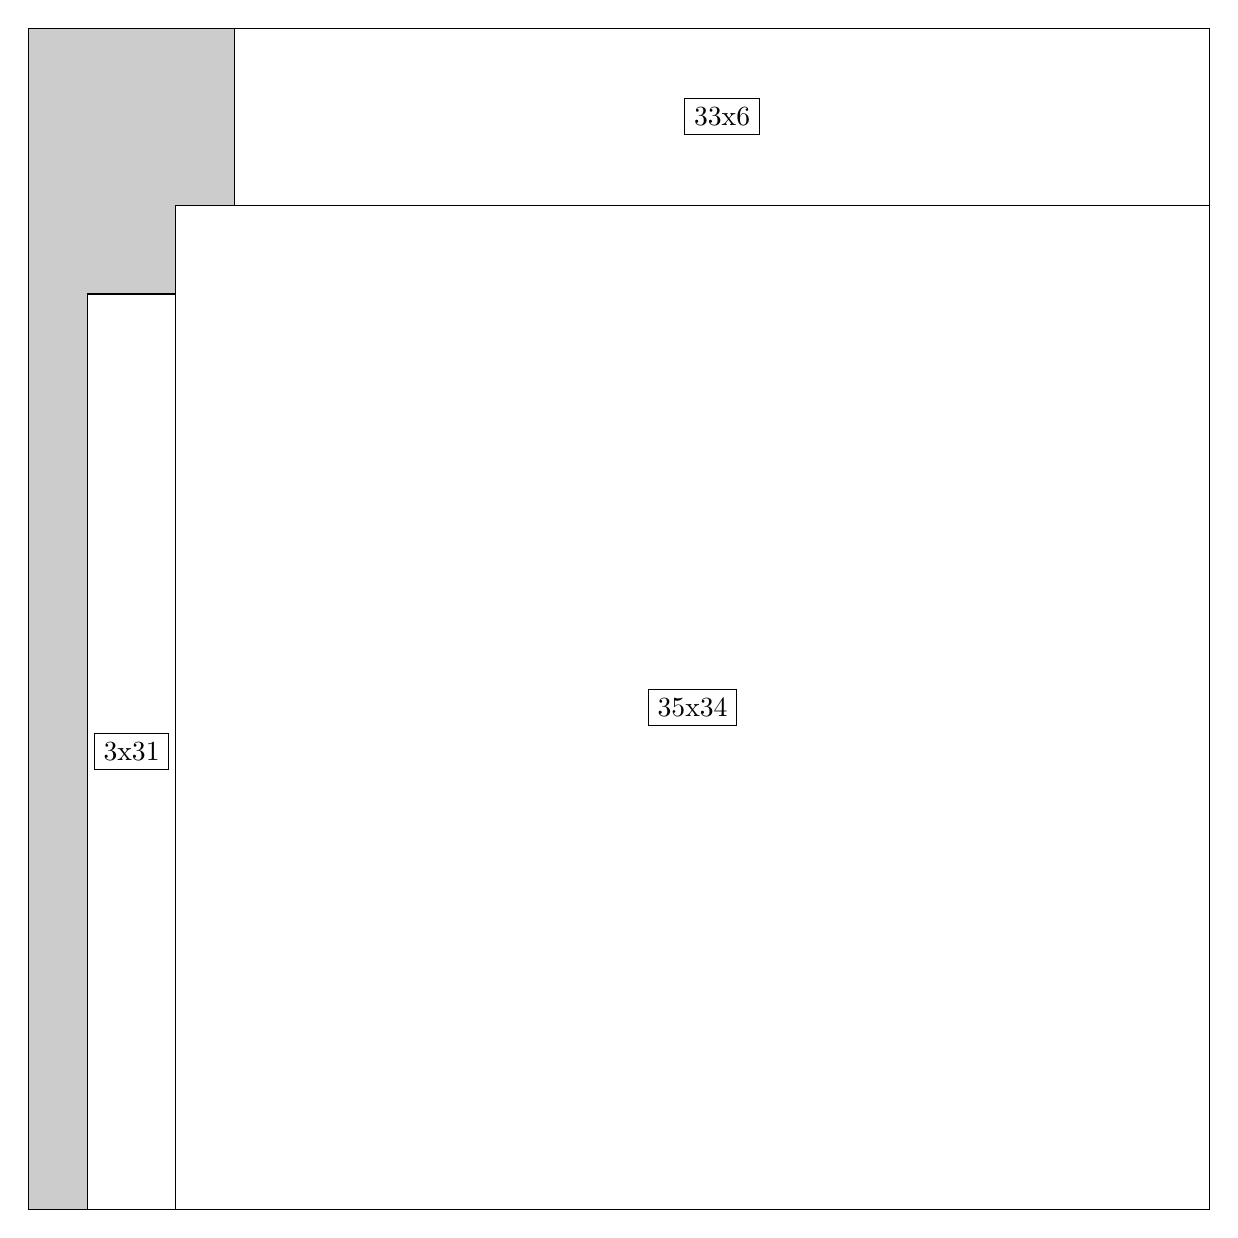
\begin{tikzpicture}[shorten >=1pt,scale=1.0,every node/.style={scale=1.0},->]
\tikzstyle{vertex}=[circle,fill=black!25,minimum size=14pt,inner sep=0pt]
\filldraw[fill=gray!40!white, draw=black] (0,0) rectangle (15.0,15.0);
\foreach \name/\x/\y/\w/\h in {35x34/1.875/0.0/13.125/12.75,3x31/0.75/0.0/1.125/11.625,33x6/2.625/12.75/12.375/2.25}
\filldraw[fill=white!40!white, draw=black] (\x,\y) rectangle node[draw] (\name) {\name} ++(\w,\h);
\end{tikzpicture}


w =35 , h =34 , x =5 , y =0 , v =1190
\par
w =3 , h =31 , x =2 , y =0 , v =93
\par
w =33 , h =6 , x =7 , y =34 , v =198
\par
\newpage


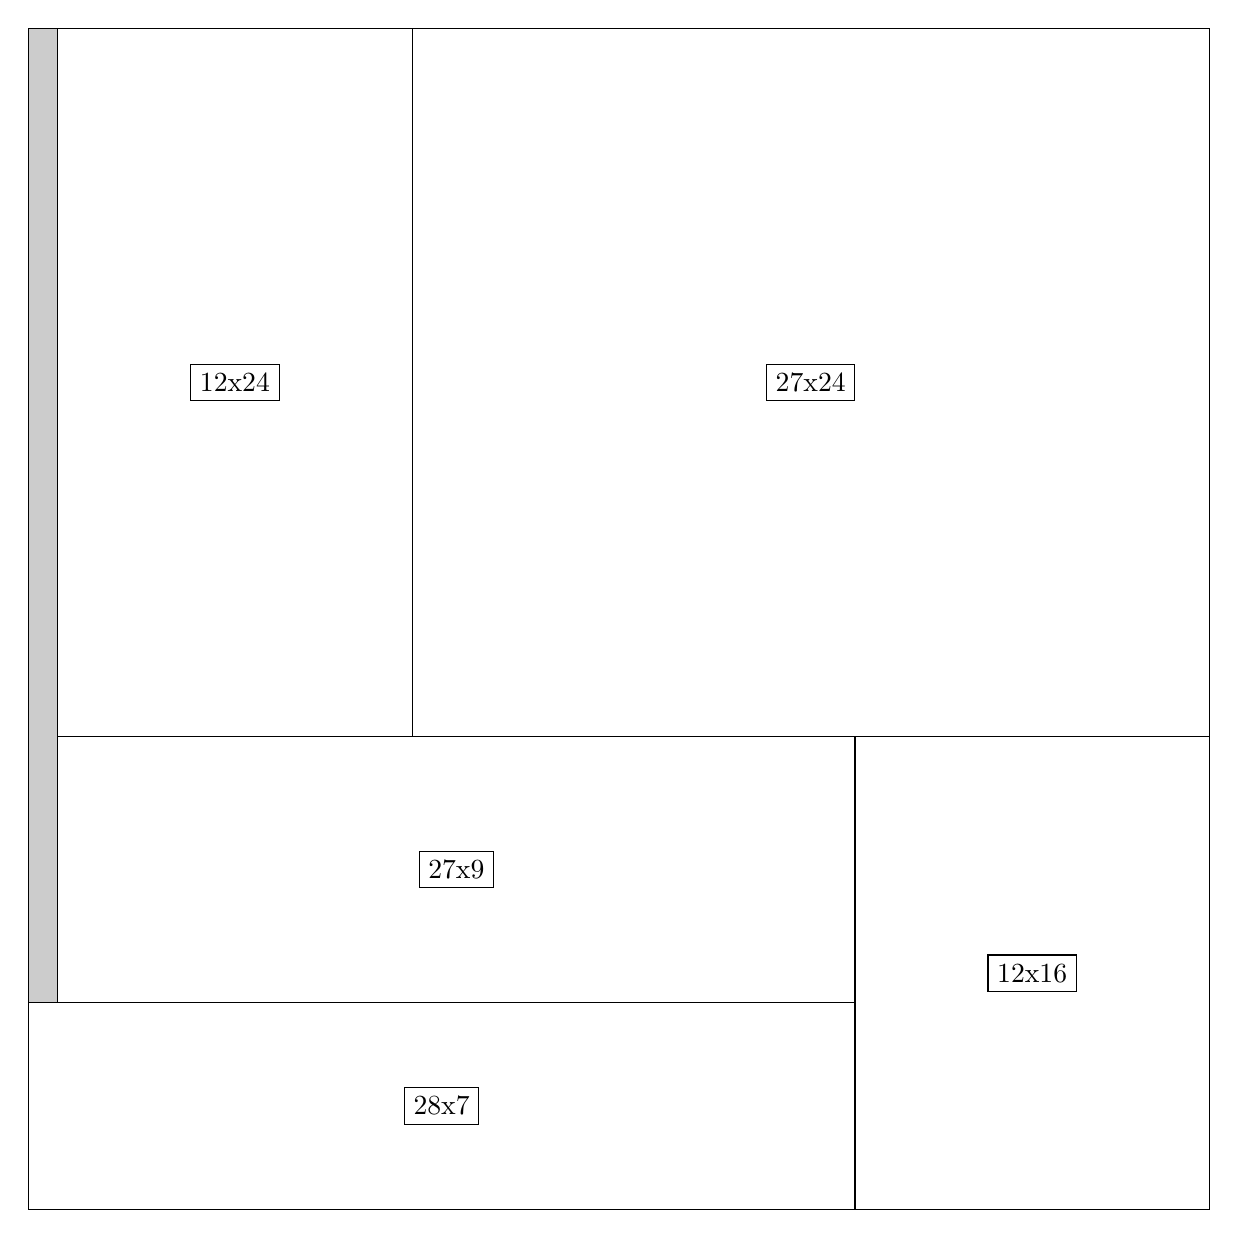
\begin{tikzpicture}[shorten >=1pt,scale=1.0,every node/.style={scale=1.0},->]
\tikzstyle{vertex}=[circle,fill=black!25,minimum size=14pt,inner sep=0pt]
\filldraw[fill=gray!40!white, draw=black] (0,0) rectangle (15.0,15.0);
\foreach \name/\x/\y/\w/\h in {12x16/10.5/0.0/4.5/6.0,28x7/0.0/0.0/10.5/2.625,27x9/0.375/2.625/10.125/3.375,27x24/4.875/6.0/10.125/9.0,12x24/0.375/6.0/4.5/9.0}
\filldraw[fill=white!40!white, draw=black] (\x,\y) rectangle node[draw] (\name) {\name} ++(\w,\h);
\end{tikzpicture}


w =12 , h =16 , x =28 , y =0 , v =192
\par
w =28 , h =7 , x =0 , y =0 , v =196
\par
w =27 , h =9 , x =1 , y =7 , v =243
\par
w =27 , h =24 , x =13 , y =16 , v =648
\par
w =12 , h =24 , x =1 , y =16 , v =288
\par
\newpage


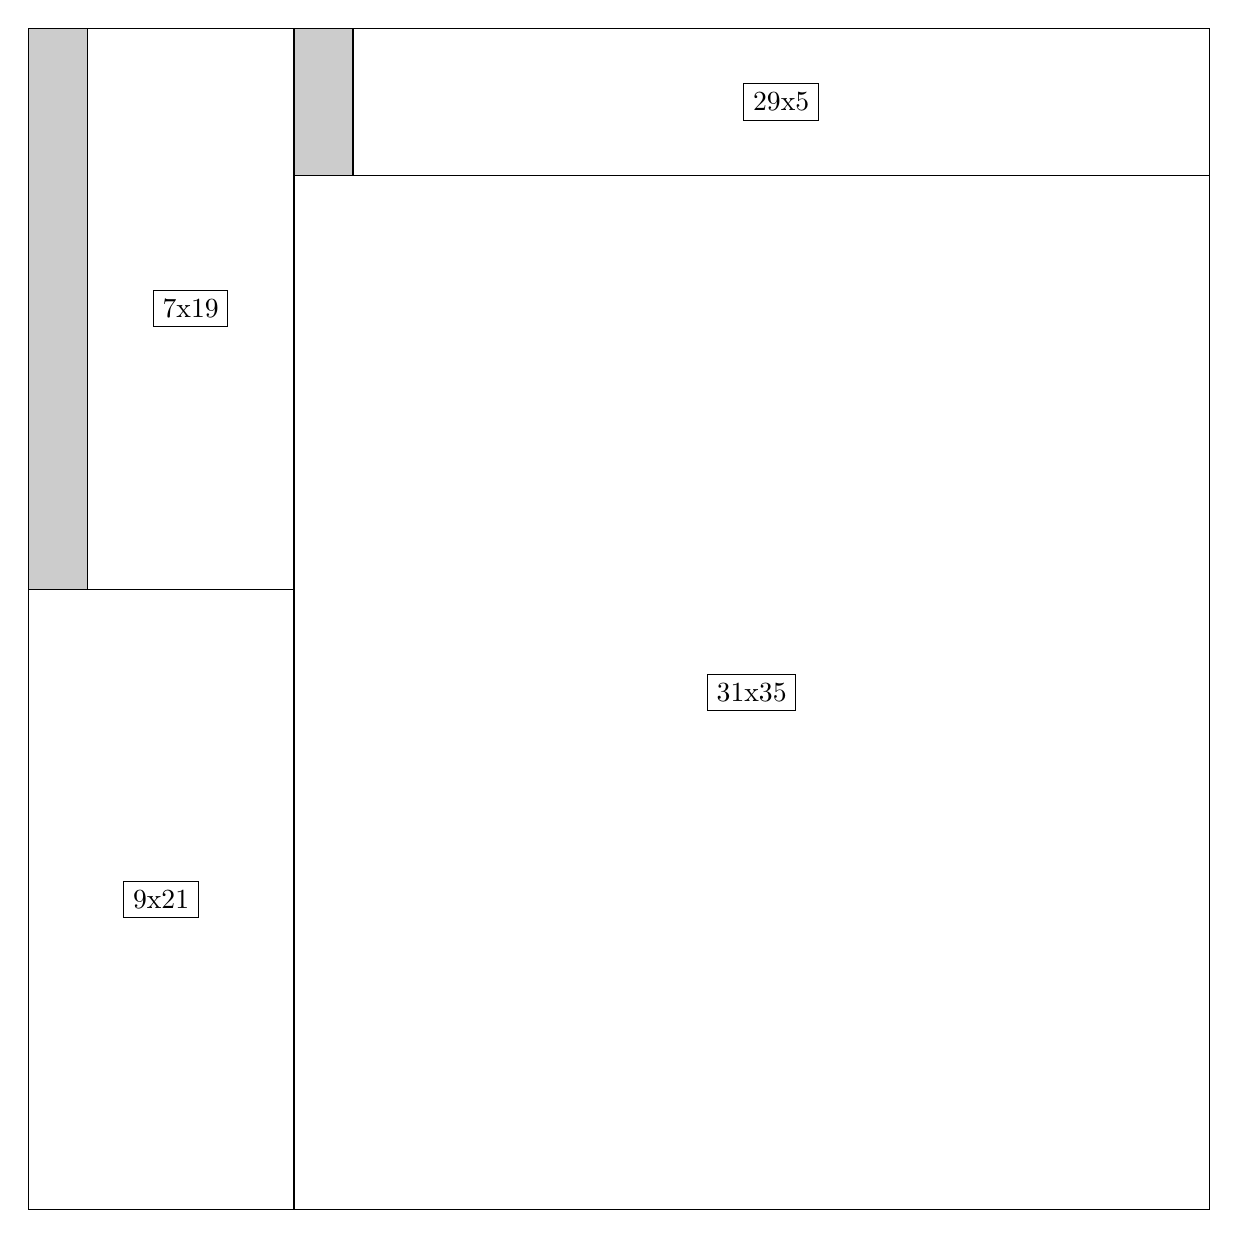
\begin{tikzpicture}[shorten >=1pt,scale=1.0,every node/.style={scale=1.0},->]
\tikzstyle{vertex}=[circle,fill=black!25,minimum size=14pt,inner sep=0pt]
\filldraw[fill=gray!40!white, draw=black] (0,0) rectangle (15.0,15.0);
\foreach \name/\x/\y/\w/\h in {31x35/3.375/0.0/11.625/13.125,29x5/4.125/13.125/10.875/1.875,9x21/0.0/0.0/3.375/7.875,7x19/0.75/7.875/2.625/7.125}
\filldraw[fill=white!40!white, draw=black] (\x,\y) rectangle node[draw] (\name) {\name} ++(\w,\h);
\end{tikzpicture}


w =31 , h =35 , x =9 , y =0 , v =1085
\par
w =29 , h =5 , x =11 , y =35 , v =145
\par
w =9 , h =21 , x =0 , y =0 , v =189
\par
w =7 , h =19 , x =2 , y =21 , v =133
\par
\newpage


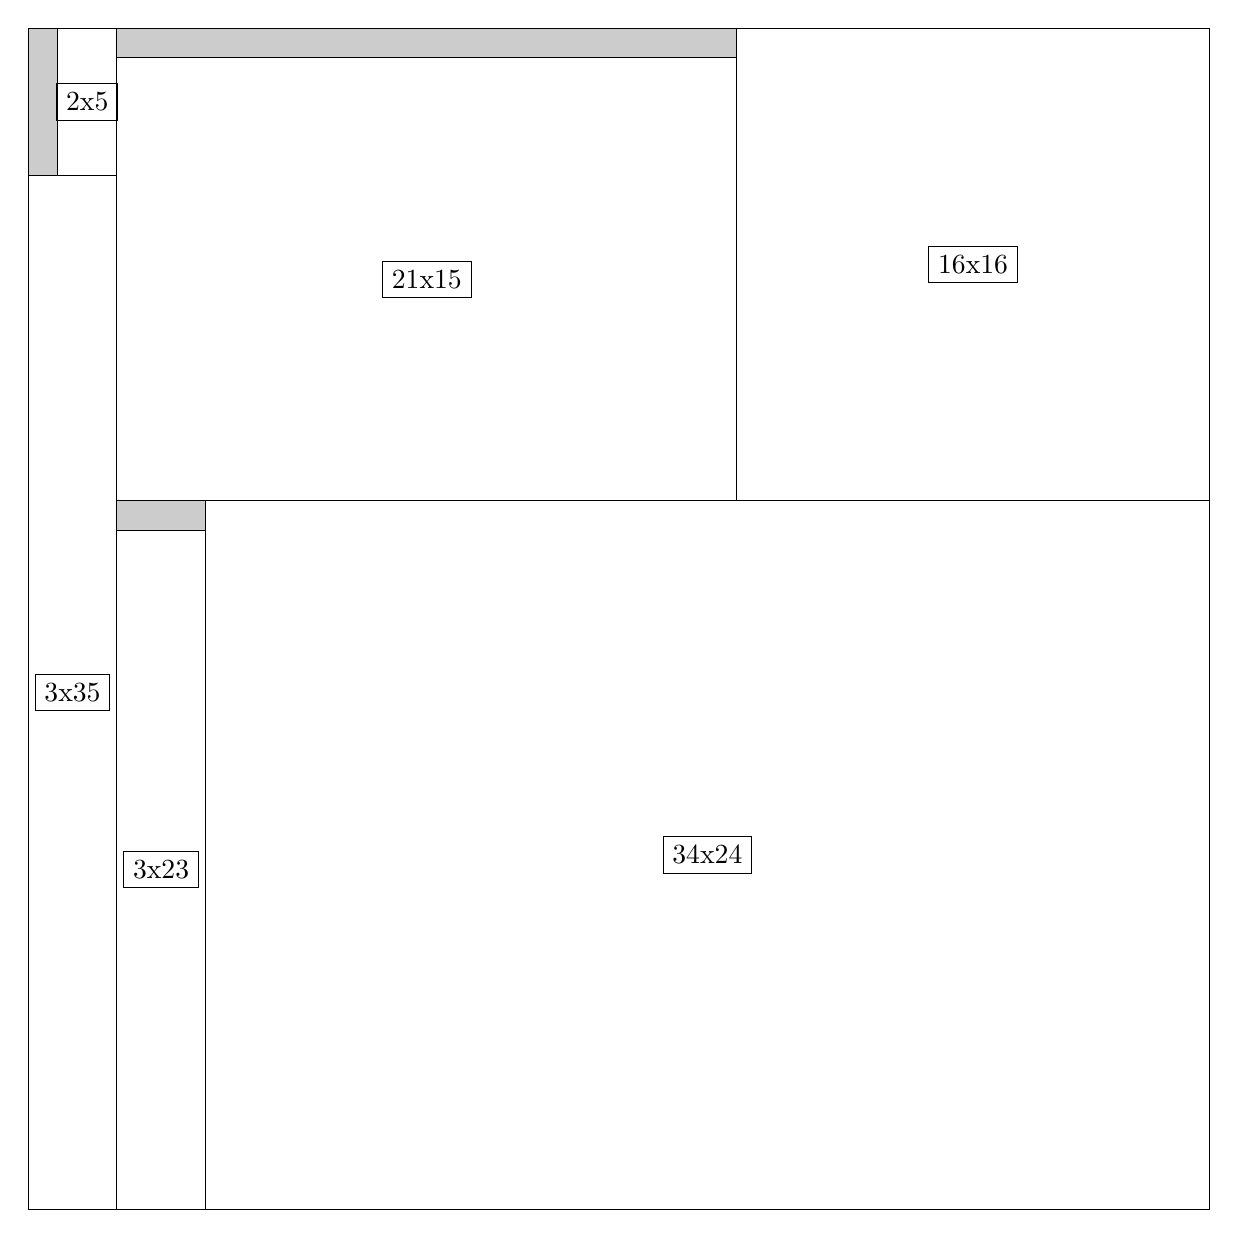
\begin{tikzpicture}[shorten >=1pt,scale=1.0,every node/.style={scale=1.0},->]
\tikzstyle{vertex}=[circle,fill=black!25,minimum size=14pt,inner sep=0pt]
\filldraw[fill=gray!40!white, draw=black] (0,0) rectangle (15.0,15.0);
\foreach \name/\x/\y/\w/\h in {34x24/2.25/0.0/12.75/9.0,3x23/1.125/0.0/1.125/8.625,16x16/9.0/9.0/6.0/6.0,21x15/1.125/9.0/7.875/5.625,3x35/0.0/0.0/1.125/13.125,2x5/0.375/13.125/0.75/1.875}
\filldraw[fill=white!40!white, draw=black] (\x,\y) rectangle node[draw] (\name) {\name} ++(\w,\h);
\end{tikzpicture}


w =34 , h =24 , x =6 , y =0 , v =816
\par
w =3 , h =23 , x =3 , y =0 , v =69
\par
w =16 , h =16 , x =24 , y =24 , v =256
\par
w =21 , h =15 , x =3 , y =24 , v =315
\par
w =3 , h =35 , x =0 , y =0 , v =105
\par
w =2 , h =5 , x =1 , y =35 , v =10
\par
\newpage


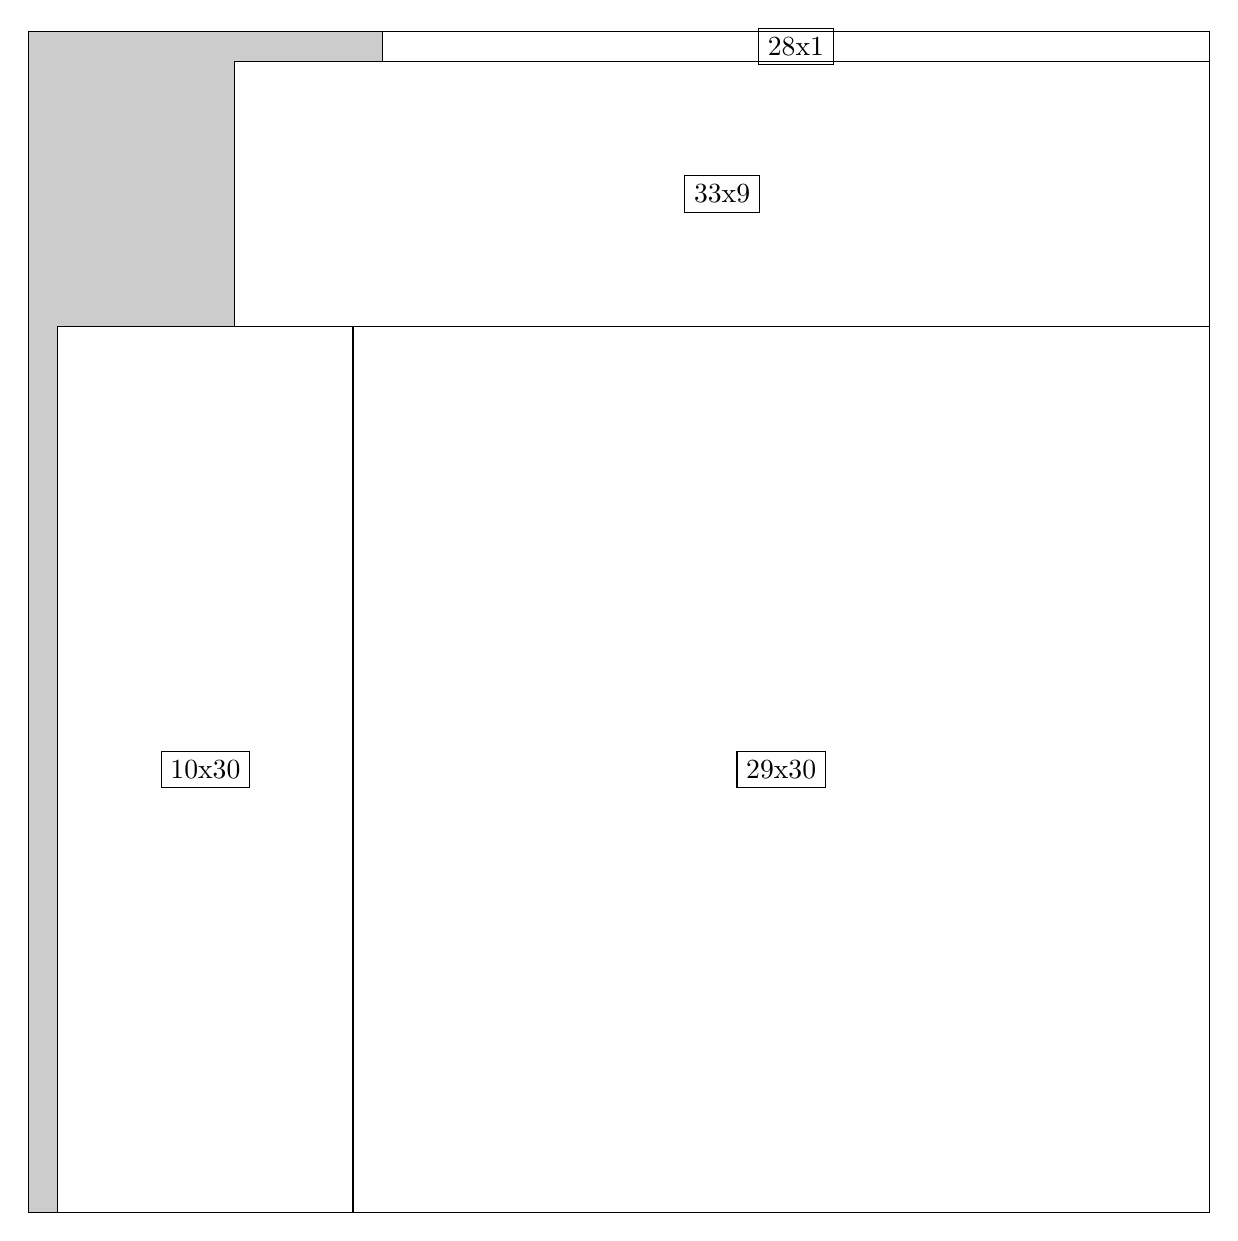
\begin{tikzpicture}[shorten >=1pt,scale=1.0,every node/.style={scale=1.0},->]
\tikzstyle{vertex}=[circle,fill=black!25,minimum size=14pt,inner sep=0pt]
\filldraw[fill=gray!40!white, draw=black] (0,0) rectangle (15.0,15.0);
\foreach \name/\x/\y/\w/\h in {29x30/4.125/0.0/10.875/11.25,10x30/0.375/0.0/3.75/11.25,33x9/2.625/11.25/12.375/3.375,28x1/4.5/14.625/10.5/0.375}
\filldraw[fill=white!40!white, draw=black] (\x,\y) rectangle node[draw] (\name) {\name} ++(\w,\h);
\end{tikzpicture}


w =29 , h =30 , x =11 , y =0 , v =870
\par
w =10 , h =30 , x =1 , y =0 , v =300
\par
w =33 , h =9 , x =7 , y =30 , v =297
\par
w =28 , h =1 , x =12 , y =39 , v =28
\par
\newpage


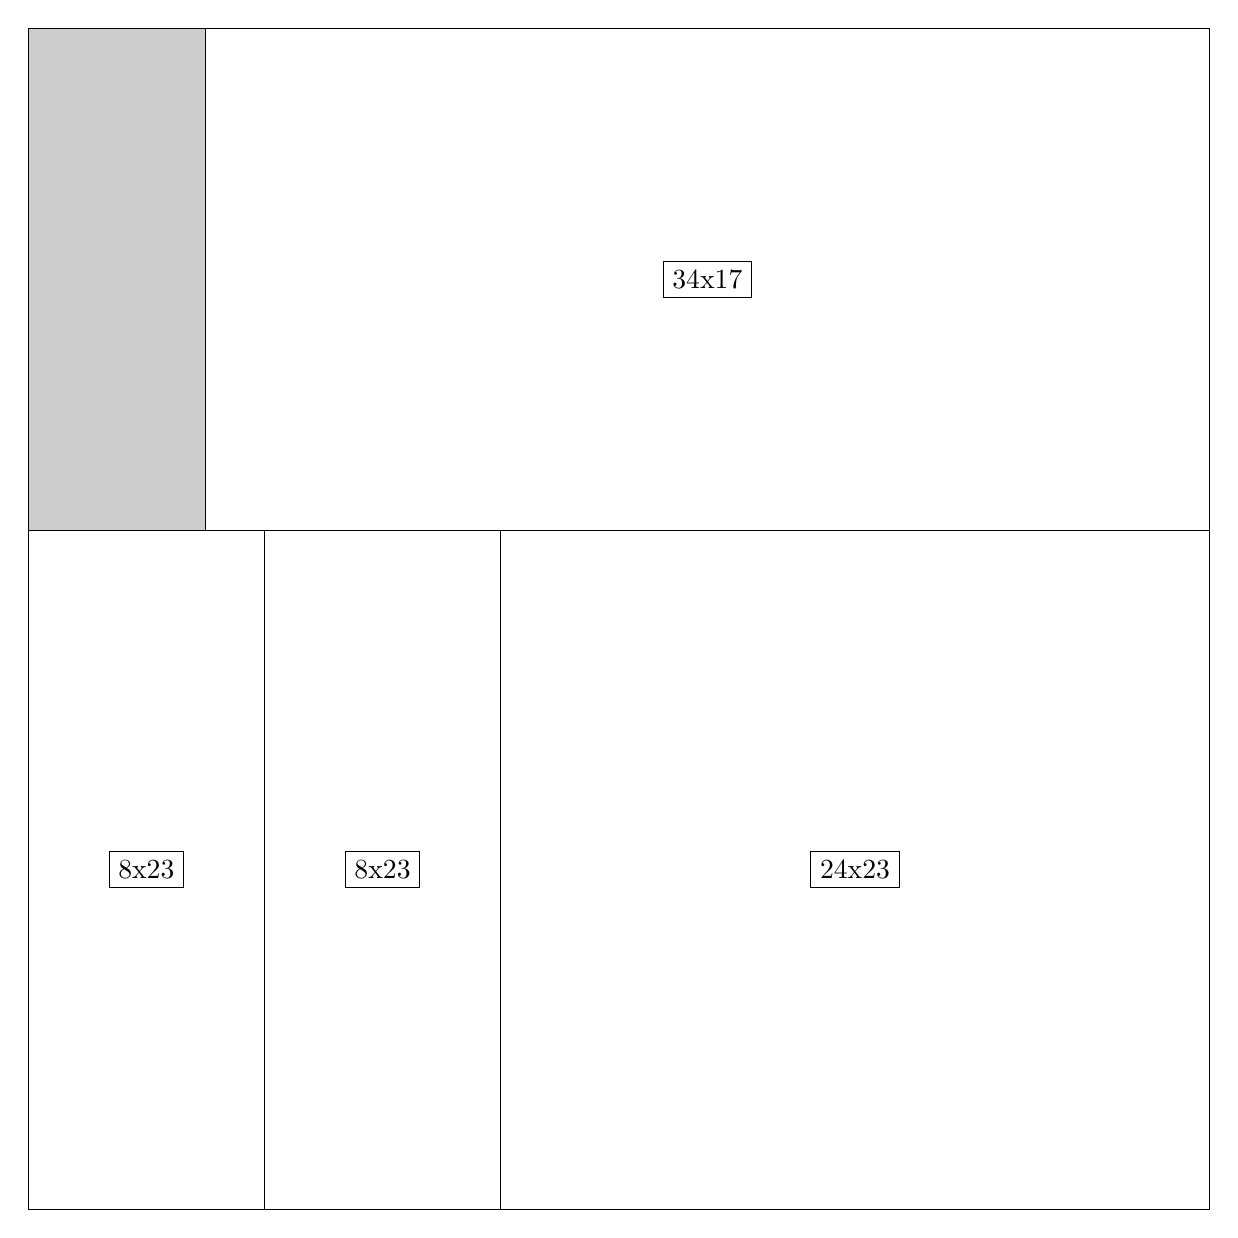
\begin{tikzpicture}[shorten >=1pt,scale=1.0,every node/.style={scale=1.0},->]
\tikzstyle{vertex}=[circle,fill=black!25,minimum size=14pt,inner sep=0pt]
\filldraw[fill=gray!40!white, draw=black] (0,0) rectangle (15.0,15.0);
\foreach \name/\x/\y/\w/\h in {24x23/6.0/0.0/9.0/8.625,8x23/3.0/0.0/3.0/8.625,8x23/0.0/0.0/3.0/8.625,34x17/2.25/8.625/12.75/6.375}
\filldraw[fill=white!40!white, draw=black] (\x,\y) rectangle node[draw] (\name) {\name} ++(\w,\h);
\end{tikzpicture}


w =24 , h =23 , x =16 , y =0 , v =552
\par
w =8 , h =23 , x =8 , y =0 , v =184
\par
w =8 , h =23 , x =0 , y =0 , v =184
\par
w =34 , h =17 , x =6 , y =23 , v =578
\par
\newpage


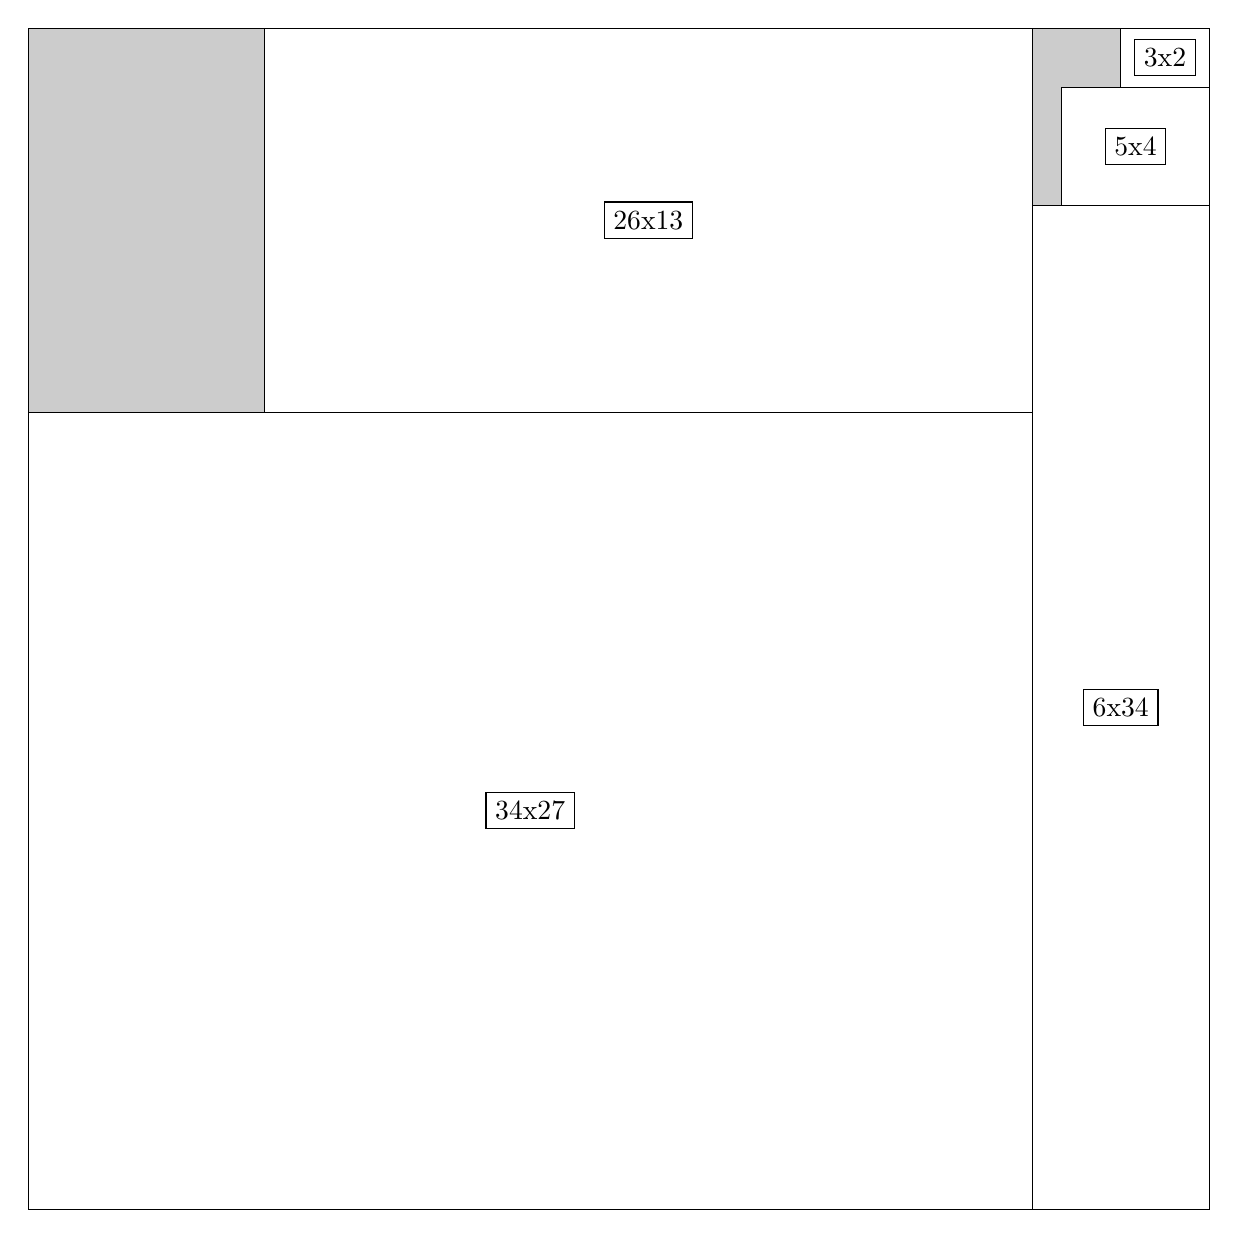
\begin{tikzpicture}[shorten >=1pt,scale=1.0,every node/.style={scale=1.0},->]
\tikzstyle{vertex}=[circle,fill=black!25,minimum size=14pt,inner sep=0pt]
\filldraw[fill=gray!40!white, draw=black] (0,0) rectangle (15.0,15.0);
\foreach \name/\x/\y/\w/\h in {6x34/12.75/0.0/2.25/12.75,5x4/13.125/12.75/1.875/1.5,3x2/13.875/14.25/1.125/0.75,34x27/0.0/0.0/12.75/10.125,26x13/3.0/10.125/9.75/4.875}
\filldraw[fill=white!40!white, draw=black] (\x,\y) rectangle node[draw] (\name) {\name} ++(\w,\h);
\end{tikzpicture}


w =6 , h =34 , x =34 , y =0 , v =204
\par
w =5 , h =4 , x =35 , y =34 , v =20
\par
w =3 , h =2 , x =37 , y =38 , v =6
\par
w =34 , h =27 , x =0 , y =0 , v =918
\par
w =26 , h =13 , x =8 , y =27 , v =338
\par
\newpage


\begin{tikzpicture}[shorten >=1pt,scale=1.0,every node/.style={scale=1.0},->]
\tikzstyle{vertex}=[circle,fill=black!25,minimum size=14pt,inner sep=0pt]
\filldraw[fill=gray!40!white, draw=black] (0,0) rectangle (15.0,15.0);
\foreach \name/\x/\y/\w/\h in {19x35/7.875/0.0/7.125/13.125,18x5/8.25/13.125/6.75/1.875,21x26/0.0/0.0/7.875/9.75,20x14/0.375/9.75/7.5/5.25}
\filldraw[fill=white!40!white, draw=black] (\x,\y) rectangle node[draw] (\name) {\name} ++(\w,\h);
\end{tikzpicture}


w =19 , h =35 , x =21 , y =0 , v =665
\par
w =18 , h =5 , x =22 , y =35 , v =90
\par
w =21 , h =26 , x =0 , y =0 , v =546
\par
w =20 , h =14 , x =1 , y =26 , v =280
\par
\newpage


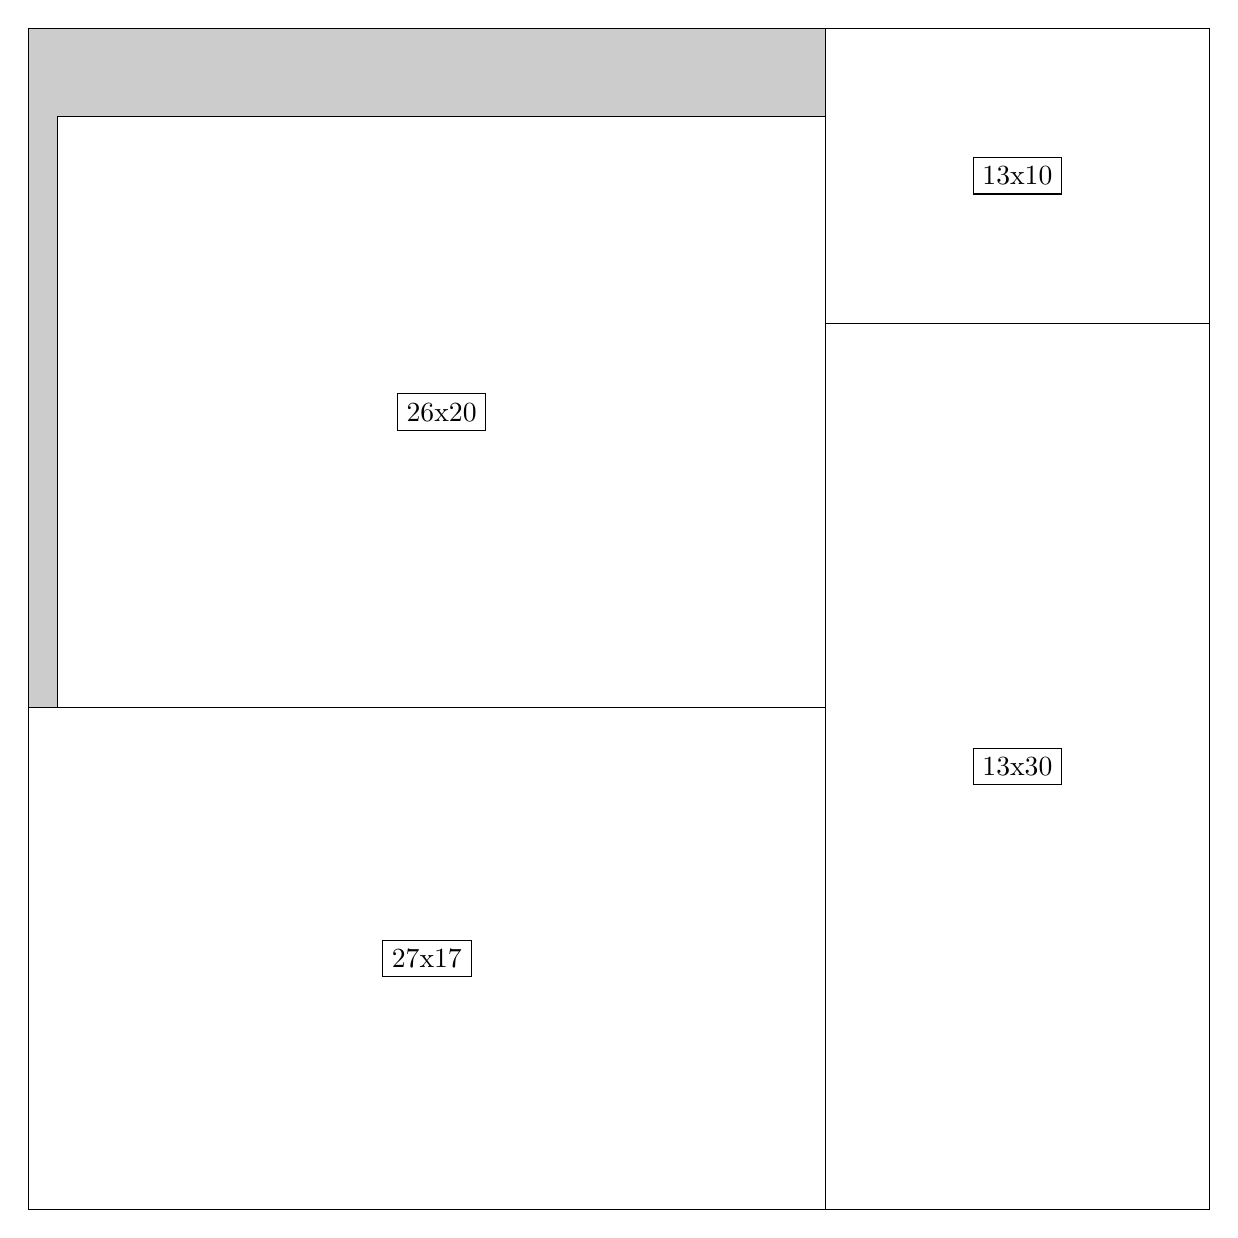
\begin{tikzpicture}[shorten >=1pt,scale=1.0,every node/.style={scale=1.0},->]
\tikzstyle{vertex}=[circle,fill=black!25,minimum size=14pt,inner sep=0pt]
\filldraw[fill=gray!40!white, draw=black] (0,0) rectangle (15.0,15.0);
\foreach \name/\x/\y/\w/\h in {13x30/10.125/0.0/4.875/11.25,13x10/10.125/11.25/4.875/3.75,27x17/0.0/0.0/10.125/6.375,26x20/0.375/6.375/9.75/7.5}
\filldraw[fill=white!40!white, draw=black] (\x,\y) rectangle node[draw] (\name) {\name} ++(\w,\h);
\end{tikzpicture}


w =13 , h =30 , x =27 , y =0 , v =390
\par
w =13 , h =10 , x =27 , y =30 , v =130
\par
w =27 , h =17 , x =0 , y =0 , v =459
\par
w =26 , h =20 , x =1 , y =17 , v =520
\par
\newpage


\begin{tikzpicture}[shorten >=1pt,scale=1.0,every node/.style={scale=1.0},->]
\tikzstyle{vertex}=[circle,fill=black!25,minimum size=14pt,inner sep=0pt]
\filldraw[fill=gray!40!white, draw=black] (0,0) rectangle (15.0,15.0);
\foreach \name/\x/\y/\w/\h in {21x23/7.125/0.0/7.875/8.625,19x22/0.0/0.0/7.125/8.25,15x1/1.5/8.25/5.625/0.375,35x17/1.875/8.625/13.125/6.375,5x15/0.0/8.625/1.875/5.625}
\filldraw[fill=white!40!white, draw=black] (\x,\y) rectangle node[draw] (\name) {\name} ++(\w,\h);
\end{tikzpicture}


w =21 , h =23 , x =19 , y =0 , v =483
\par
w =19 , h =22 , x =0 , y =0 , v =418
\par
w =15 , h =1 , x =4 , y =22 , v =15
\par
w =35 , h =17 , x =5 , y =23 , v =595
\par
w =5 , h =15 , x =0 , y =23 , v =75
\par
\newpage


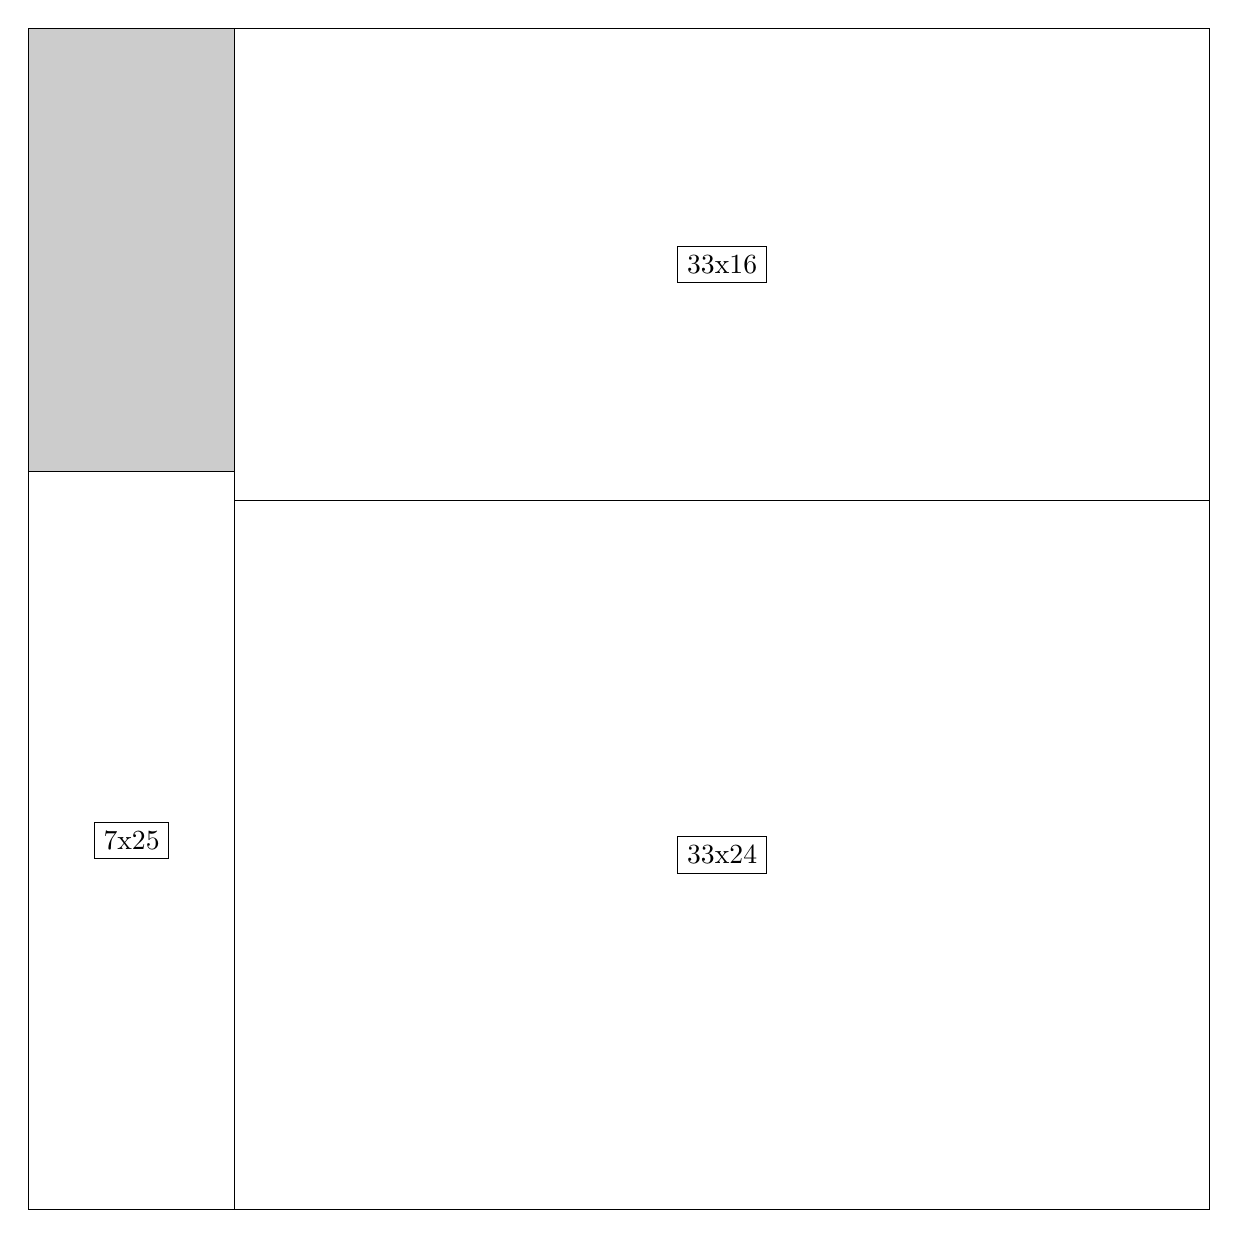
\begin{tikzpicture}[shorten >=1pt,scale=1.0,every node/.style={scale=1.0},->]
\tikzstyle{vertex}=[circle,fill=black!25,minimum size=14pt,inner sep=0pt]
\filldraw[fill=gray!40!white, draw=black] (0,0) rectangle (15.0,15.0);
\foreach \name/\x/\y/\w/\h in {33x24/2.625/0.0/12.375/9.0,33x16/2.625/9.0/12.375/6.0,7x25/0.0/0.0/2.625/9.375}
\filldraw[fill=white!40!white, draw=black] (\x,\y) rectangle node[draw] (\name) {\name} ++(\w,\h);
\end{tikzpicture}


w =33 , h =24 , x =7 , y =0 , v =792
\par
w =33 , h =16 , x =7 , y =24 , v =528
\par
w =7 , h =25 , x =0 , y =0 , v =175
\par
\newpage


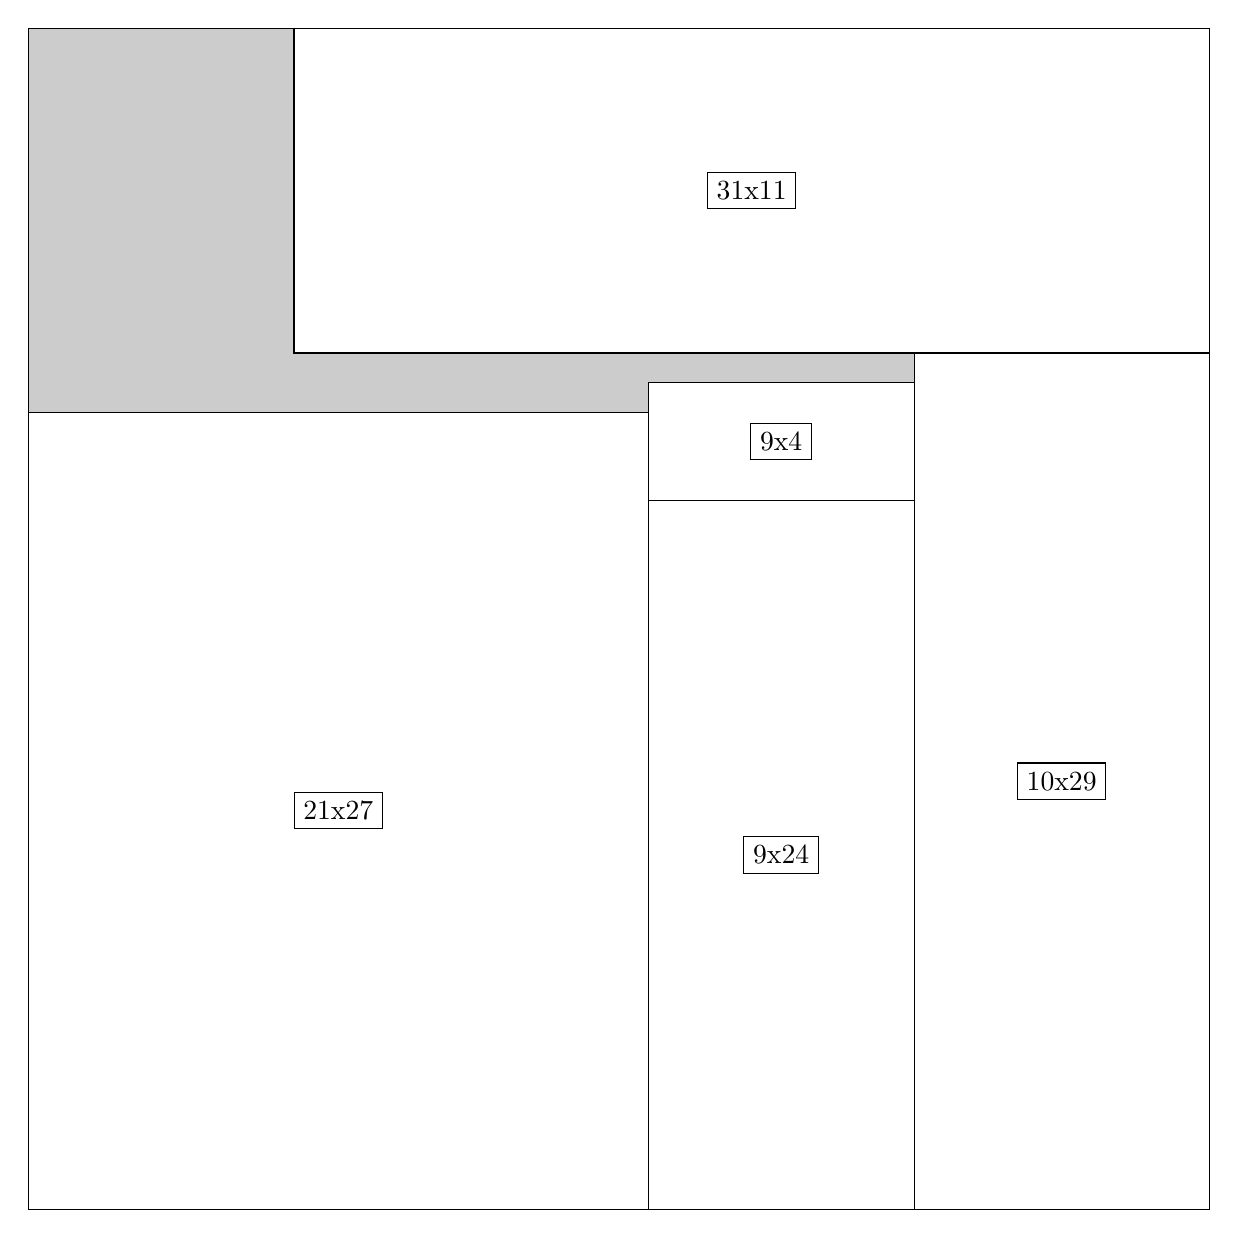
\begin{tikzpicture}[shorten >=1pt,scale=1.0,every node/.style={scale=1.0},->]
\tikzstyle{vertex}=[circle,fill=black!25,minimum size=14pt,inner sep=0pt]
\filldraw[fill=gray!40!white, draw=black] (0,0) rectangle (15.0,15.0);
\foreach \name/\x/\y/\w/\h in {10x29/11.25/0.0/3.75/10.875,9x24/7.875/0.0/3.375/9.0,9x4/7.875/9.0/3.375/1.5,21x27/0.0/0.0/7.875/10.125,31x11/3.375/10.875/11.625/4.125}
\filldraw[fill=white!40!white, draw=black] (\x,\y) rectangle node[draw] (\name) {\name} ++(\w,\h);
\end{tikzpicture}


w =10 , h =29 , x =30 , y =0 , v =290
\par
w =9 , h =24 , x =21 , y =0 , v =216
\par
w =9 , h =4 , x =21 , y =24 , v =36
\par
w =21 , h =27 , x =0 , y =0 , v =567
\par
w =31 , h =11 , x =9 , y =29 , v =341
\par
\newpage


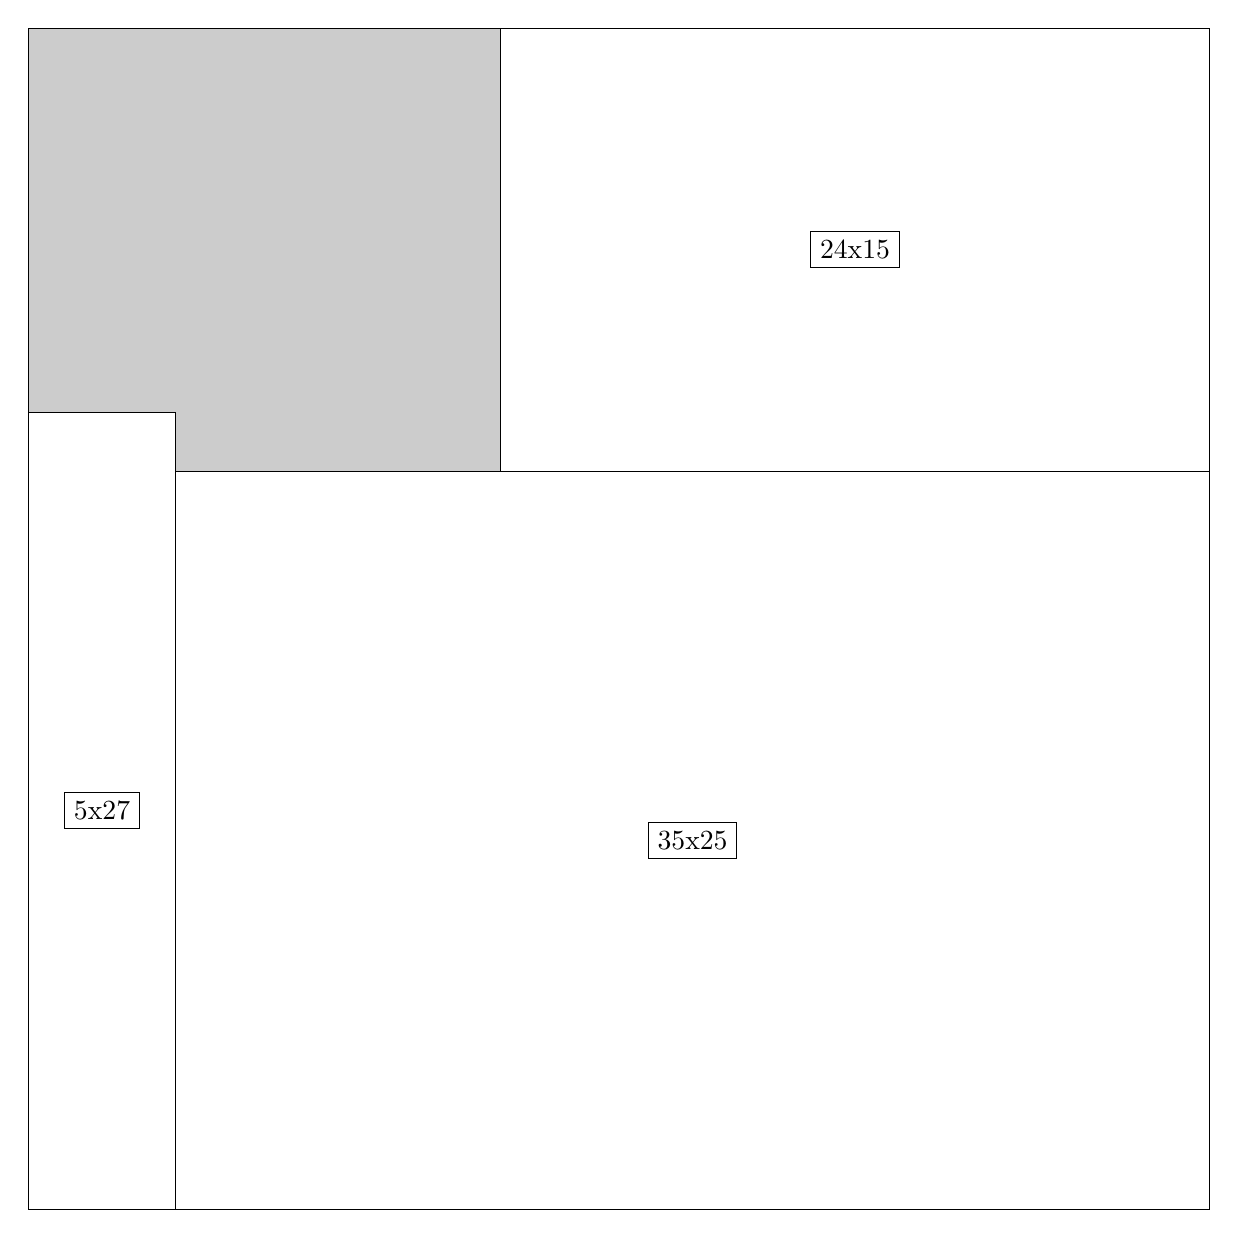
\begin{tikzpicture}[shorten >=1pt,scale=1.0,every node/.style={scale=1.0},->]
\tikzstyle{vertex}=[circle,fill=black!25,minimum size=14pt,inner sep=0pt]
\filldraw[fill=gray!40!white, draw=black] (0,0) rectangle (15.0,15.0);
\foreach \name/\x/\y/\w/\h in {35x25/1.875/0.0/13.125/9.375,24x15/6.0/9.375/9.0/5.625,5x27/0.0/0.0/1.875/10.125}
\filldraw[fill=white!40!white, draw=black] (\x,\y) rectangle node[draw] (\name) {\name} ++(\w,\h);
\end{tikzpicture}


w =35 , h =25 , x =5 , y =0 , v =875
\par
w =24 , h =15 , x =16 , y =25 , v =360
\par
w =5 , h =27 , x =0 , y =0 , v =135
\par
\newpage


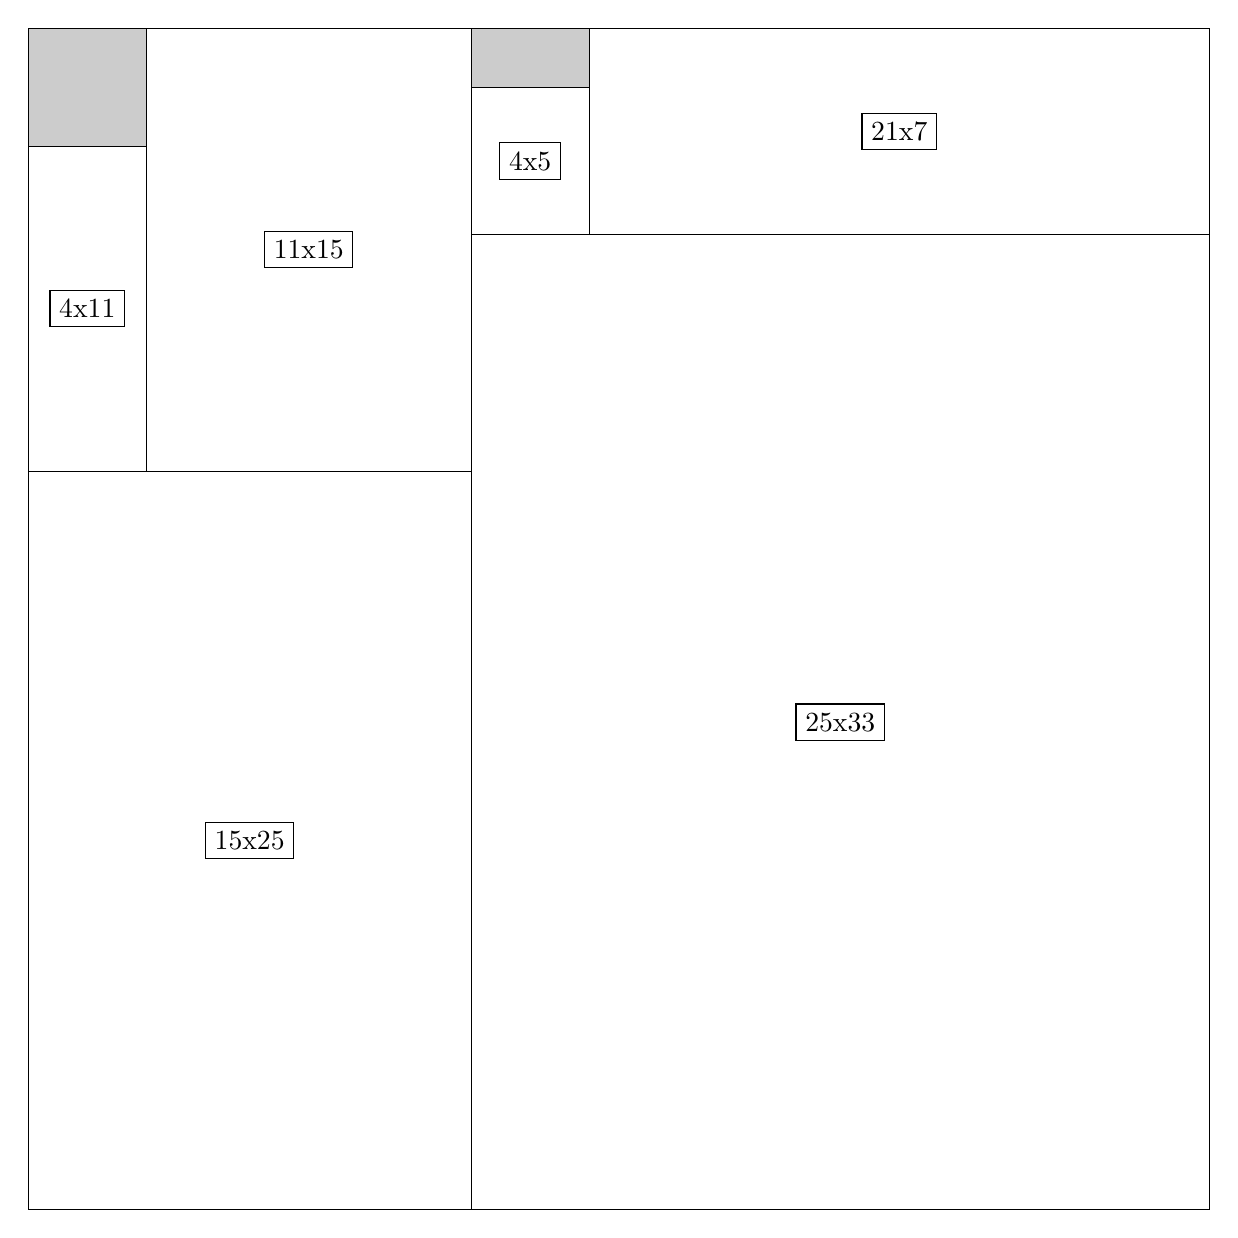
\begin{tikzpicture}[shorten >=1pt,scale=1.0,every node/.style={scale=1.0},->]
\tikzstyle{vertex}=[circle,fill=black!25,minimum size=14pt,inner sep=0pt]
\filldraw[fill=gray!40!white, draw=black] (0,0) rectangle (15.0,15.0);
\foreach \name/\x/\y/\w/\h in {25x33/5.625/0.0/9.375/12.375,21x7/7.125/12.375/7.875/2.625,4x5/5.625/12.375/1.5/1.875,15x25/0.0/0.0/5.625/9.375,11x15/1.5/9.375/4.125/5.625,4x11/0.0/9.375/1.5/4.125}
\filldraw[fill=white!40!white, draw=black] (\x,\y) rectangle node[draw] (\name) {\name} ++(\w,\h);
\end{tikzpicture}


w =25 , h =33 , x =15 , y =0 , v =825
\par
w =21 , h =7 , x =19 , y =33 , v =147
\par
w =4 , h =5 , x =15 , y =33 , v =20
\par
w =15 , h =25 , x =0 , y =0 , v =375
\par
w =11 , h =15 , x =4 , y =25 , v =165
\par
w =4 , h =11 , x =0 , y =25 , v =44
\par
\newpage


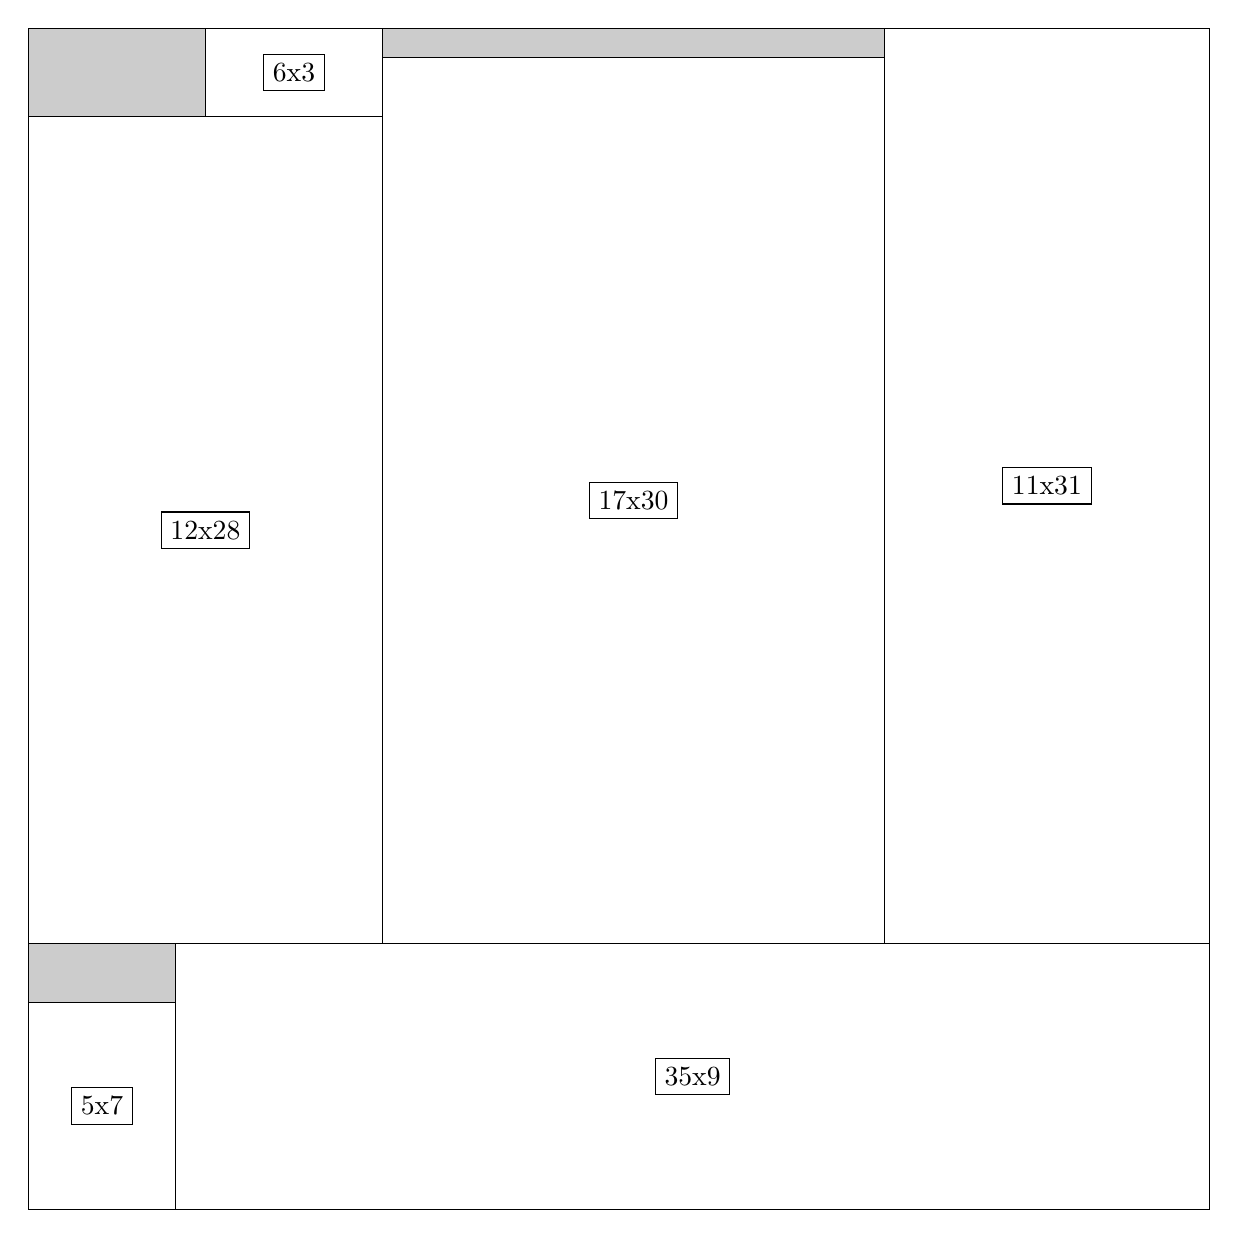
\begin{tikzpicture}[shorten >=1pt,scale=1.0,every node/.style={scale=1.0},->]
\tikzstyle{vertex}=[circle,fill=black!25,minimum size=14pt,inner sep=0pt]
\filldraw[fill=gray!40!white, draw=black] (0,0) rectangle (15.0,15.0);
\foreach \name/\x/\y/\w/\h in {35x9/1.875/0.0/13.125/3.375,5x7/0.0/0.0/1.875/2.625,11x31/10.875/3.375/4.125/11.625,17x30/4.5/3.375/6.375/11.25,12x28/0.0/3.375/4.5/10.5,6x3/2.25/13.875/2.25/1.125}
\filldraw[fill=white!40!white, draw=black] (\x,\y) rectangle node[draw] (\name) {\name} ++(\w,\h);
\end{tikzpicture}


w =35 , h =9 , x =5 , y =0 , v =315
\par
w =5 , h =7 , x =0 , y =0 , v =35
\par
w =11 , h =31 , x =29 , y =9 , v =341
\par
w =17 , h =30 , x =12 , y =9 , v =510
\par
w =12 , h =28 , x =0 , y =9 , v =336
\par
w =6 , h =3 , x =6 , y =37 , v =18
\par
\newpage


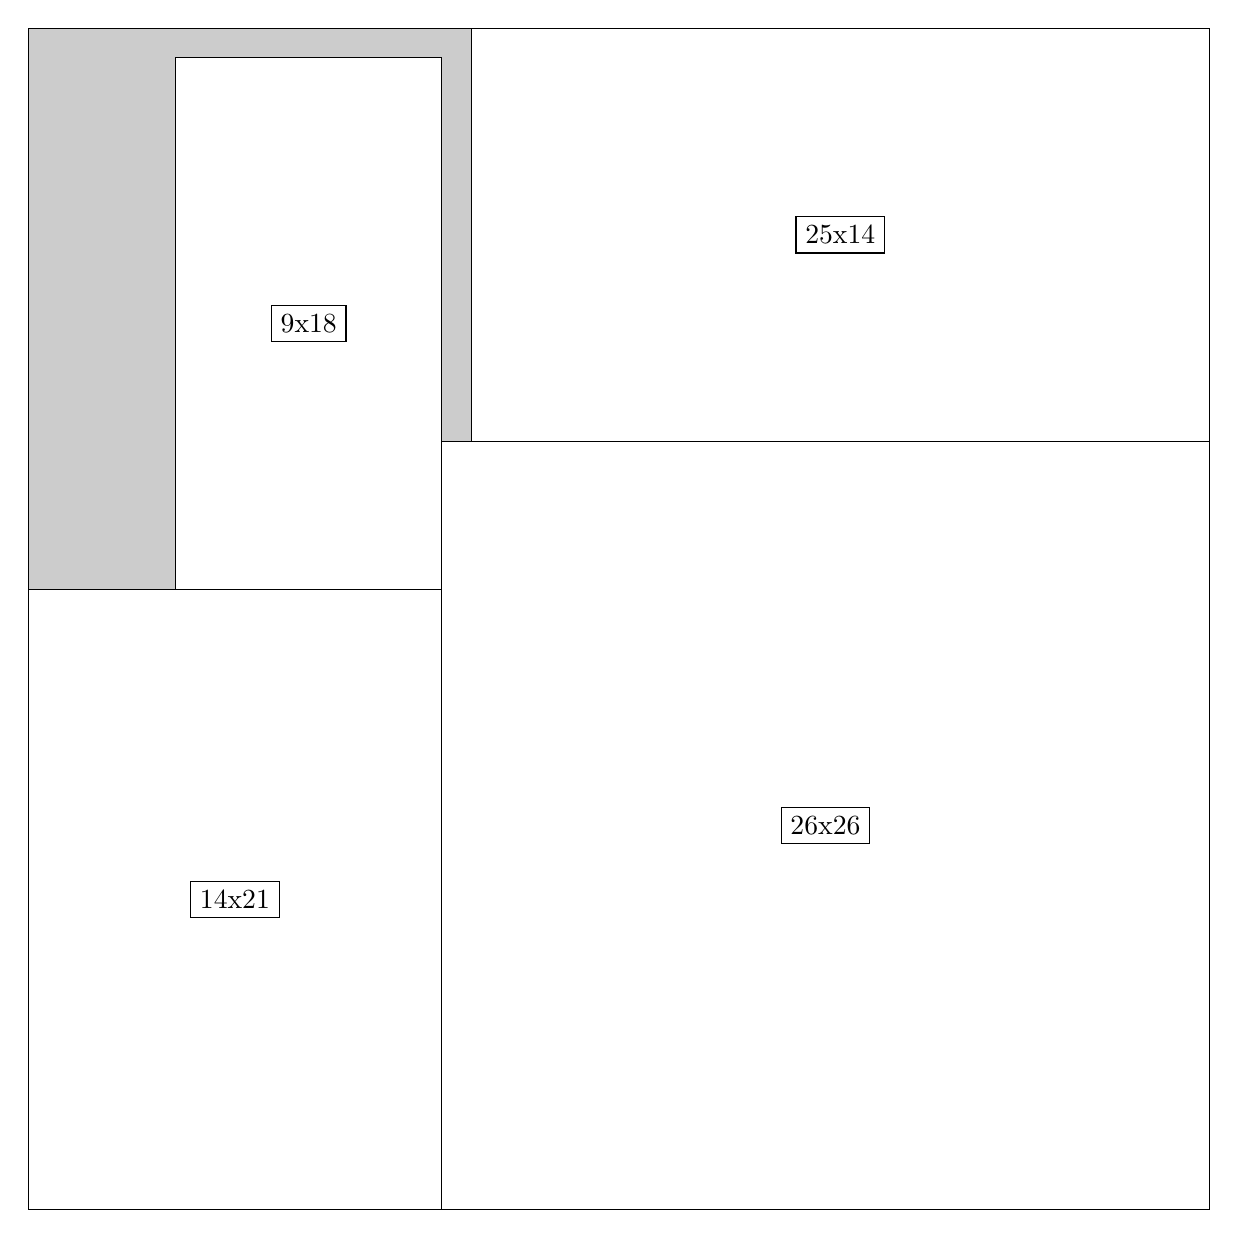
\begin{tikzpicture}[shorten >=1pt,scale=1.0,every node/.style={scale=1.0},->]
\tikzstyle{vertex}=[circle,fill=black!25,minimum size=14pt,inner sep=0pt]
\filldraw[fill=gray!40!white, draw=black] (0,0) rectangle (15.0,15.0);
\foreach \name/\x/\y/\w/\h in {26x26/5.25/0.0/9.75/9.75,25x14/5.625/9.75/9.375/5.25,14x21/0.0/0.0/5.25/7.875,9x18/1.875/7.875/3.375/6.75}
\filldraw[fill=white!40!white, draw=black] (\x,\y) rectangle node[draw] (\name) {\name} ++(\w,\h);
\end{tikzpicture}


w =26 , h =26 , x =14 , y =0 , v =676
\par
w =25 , h =14 , x =15 , y =26 , v =350
\par
w =14 , h =21 , x =0 , y =0 , v =294
\par
w =9 , h =18 , x =5 , y =21 , v =162
\par
\newpage


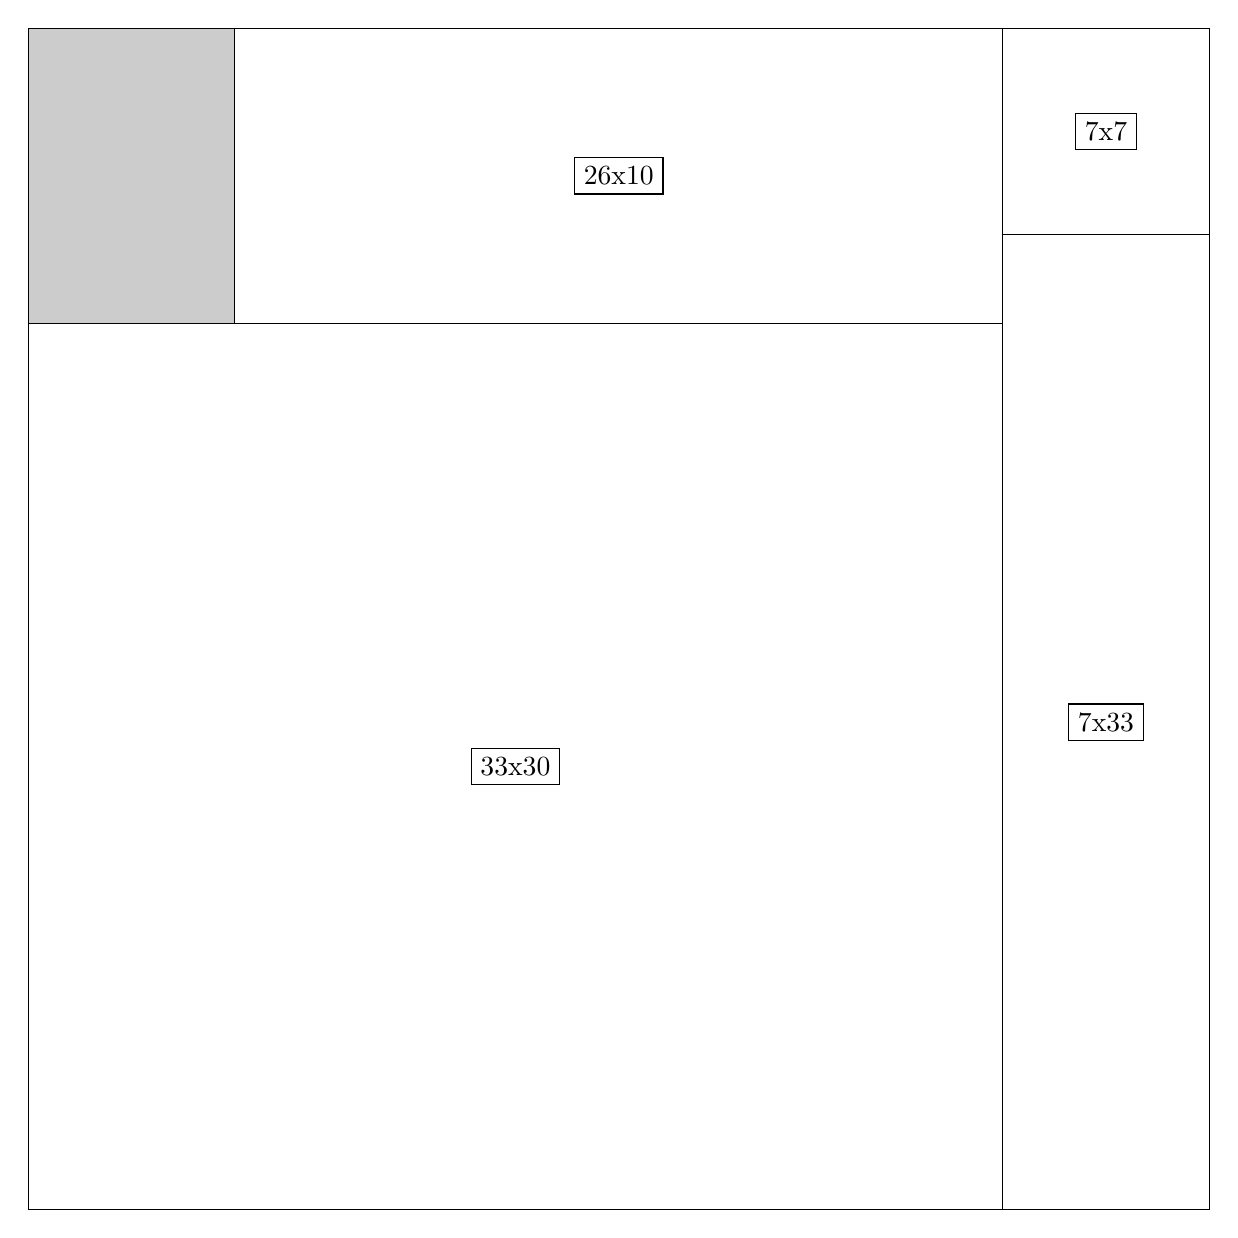
\begin{tikzpicture}[shorten >=1pt,scale=1.0,every node/.style={scale=1.0},->]
\tikzstyle{vertex}=[circle,fill=black!25,minimum size=14pt,inner sep=0pt]
\filldraw[fill=gray!40!white, draw=black] (0,0) rectangle (15.0,15.0);
\foreach \name/\x/\y/\w/\h in {7x33/12.375/0.0/2.625/12.375,7x7/12.375/12.375/2.625/2.625,33x30/0.0/0.0/12.375/11.25,26x10/2.625/11.25/9.75/3.75}
\filldraw[fill=white!40!white, draw=black] (\x,\y) rectangle node[draw] (\name) {\name} ++(\w,\h);
\end{tikzpicture}


w =7 , h =33 , x =33 , y =0 , v =231
\par
w =7 , h =7 , x =33 , y =33 , v =49
\par
w =33 , h =30 , x =0 , y =0 , v =990
\par
w =26 , h =10 , x =7 , y =30 , v =260
\par
\newpage


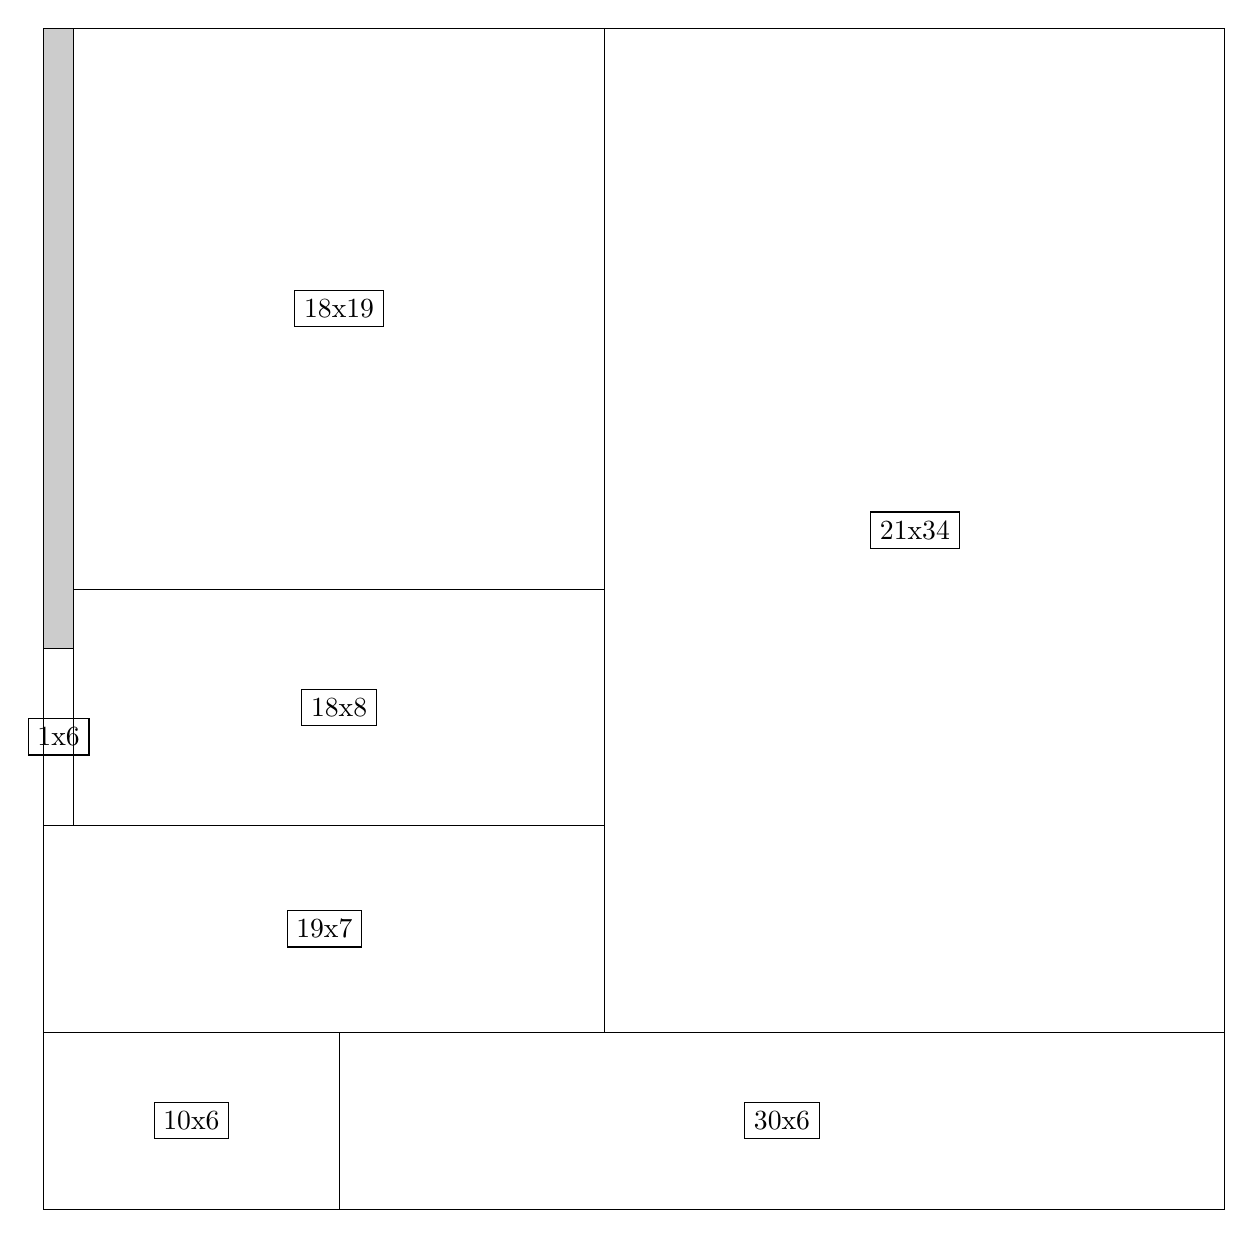
\begin{tikzpicture}[shorten >=1pt,scale=1.0,every node/.style={scale=1.0},->]
\tikzstyle{vertex}=[circle,fill=black!25,minimum size=14pt,inner sep=0pt]
\filldraw[fill=gray!40!white, draw=black] (0,0) rectangle (15.0,15.0);
\foreach \name/\x/\y/\w/\h in {30x6/3.75/0.0/11.25/2.25,10x6/0.0/0.0/3.75/2.25,21x34/7.125/2.25/7.875/12.75,19x7/0.0/2.25/7.125/2.625,18x8/0.375/4.875/6.75/3.0,1x6/0.0/4.875/0.375/2.25,18x19/0.375/7.875/6.75/7.125}
\filldraw[fill=white!40!white, draw=black] (\x,\y) rectangle node[draw] (\name) {\name} ++(\w,\h);
\end{tikzpicture}


w =30 , h =6 , x =10 , y =0 , v =180
\par
w =10 , h =6 , x =0 , y =0 , v =60
\par
w =21 , h =34 , x =19 , y =6 , v =714
\par
w =19 , h =7 , x =0 , y =6 , v =133
\par
w =18 , h =8 , x =1 , y =13 , v =144
\par
w =1 , h =6 , x =0 , y =13 , v =6
\par
w =18 , h =19 , x =1 , y =21 , v =342
\par
\newpage


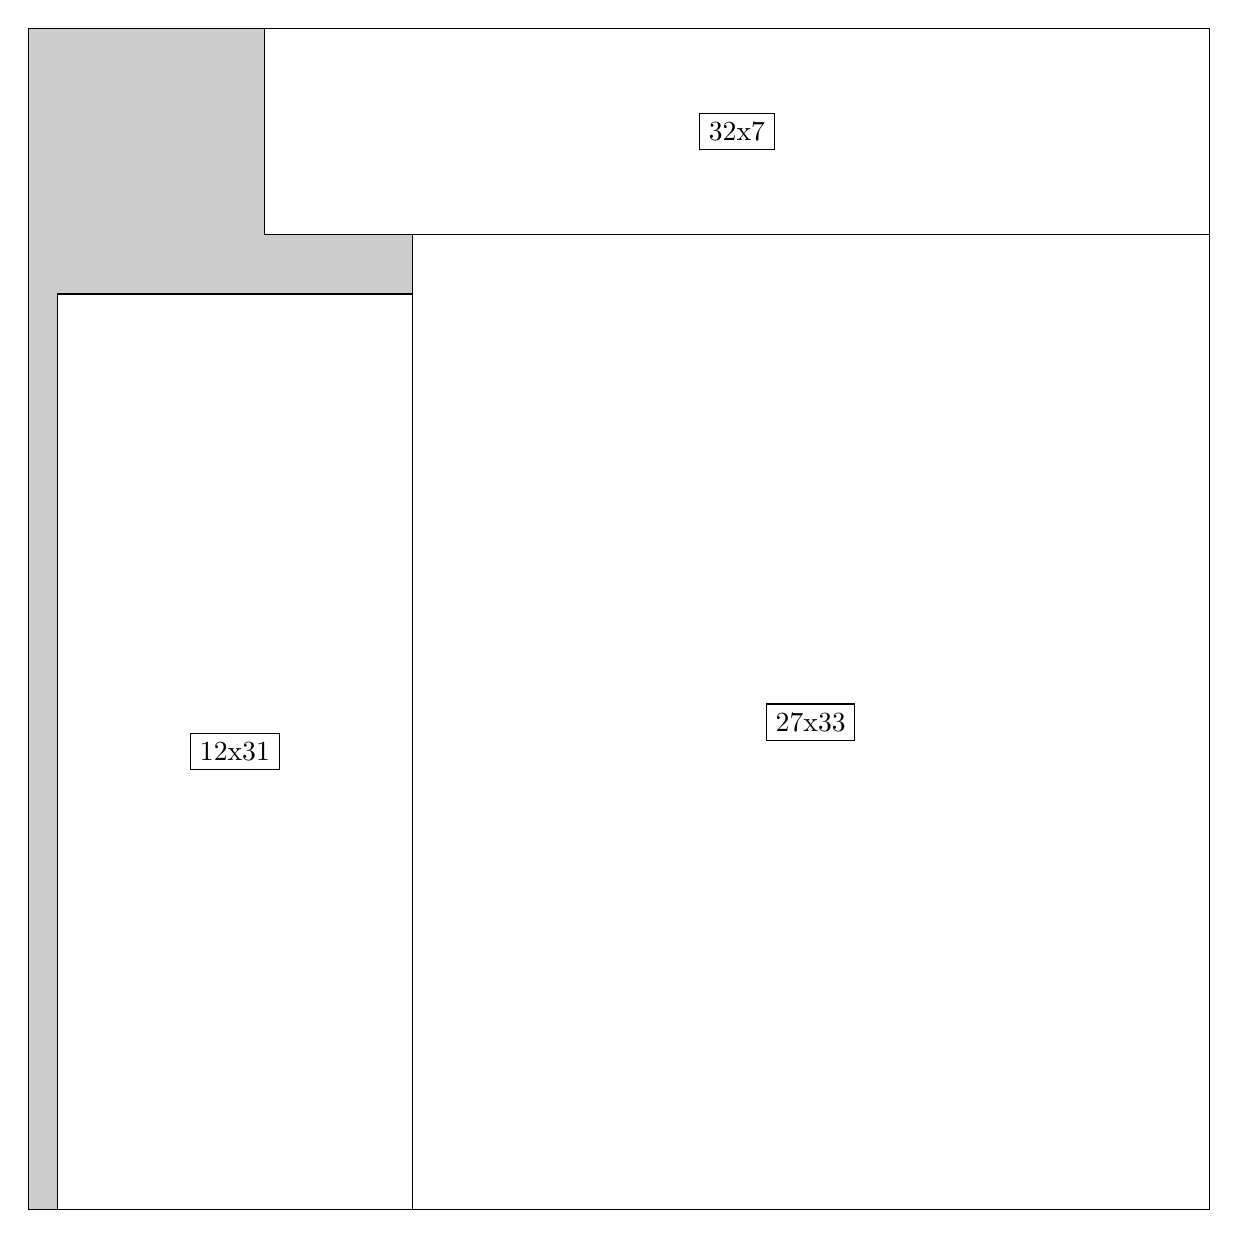
\begin{tikzpicture}[shorten >=1pt,scale=1.0,every node/.style={scale=1.0},->]
\tikzstyle{vertex}=[circle,fill=black!25,minimum size=14pt,inner sep=0pt]
\filldraw[fill=gray!40!white, draw=black] (0,0) rectangle (15.0,15.0);
\foreach \name/\x/\y/\w/\h in {27x33/4.875/0.0/10.125/12.375,12x31/0.375/0.0/4.5/11.625,32x7/3.0/12.375/12.0/2.625}
\filldraw[fill=white!40!white, draw=black] (\x,\y) rectangle node[draw] (\name) {\name} ++(\w,\h);
\end{tikzpicture}


w =27 , h =33 , x =13 , y =0 , v =891
\par
w =12 , h =31 , x =1 , y =0 , v =372
\par
w =32 , h =7 , x =8 , y =33 , v =224
\par
\newpage


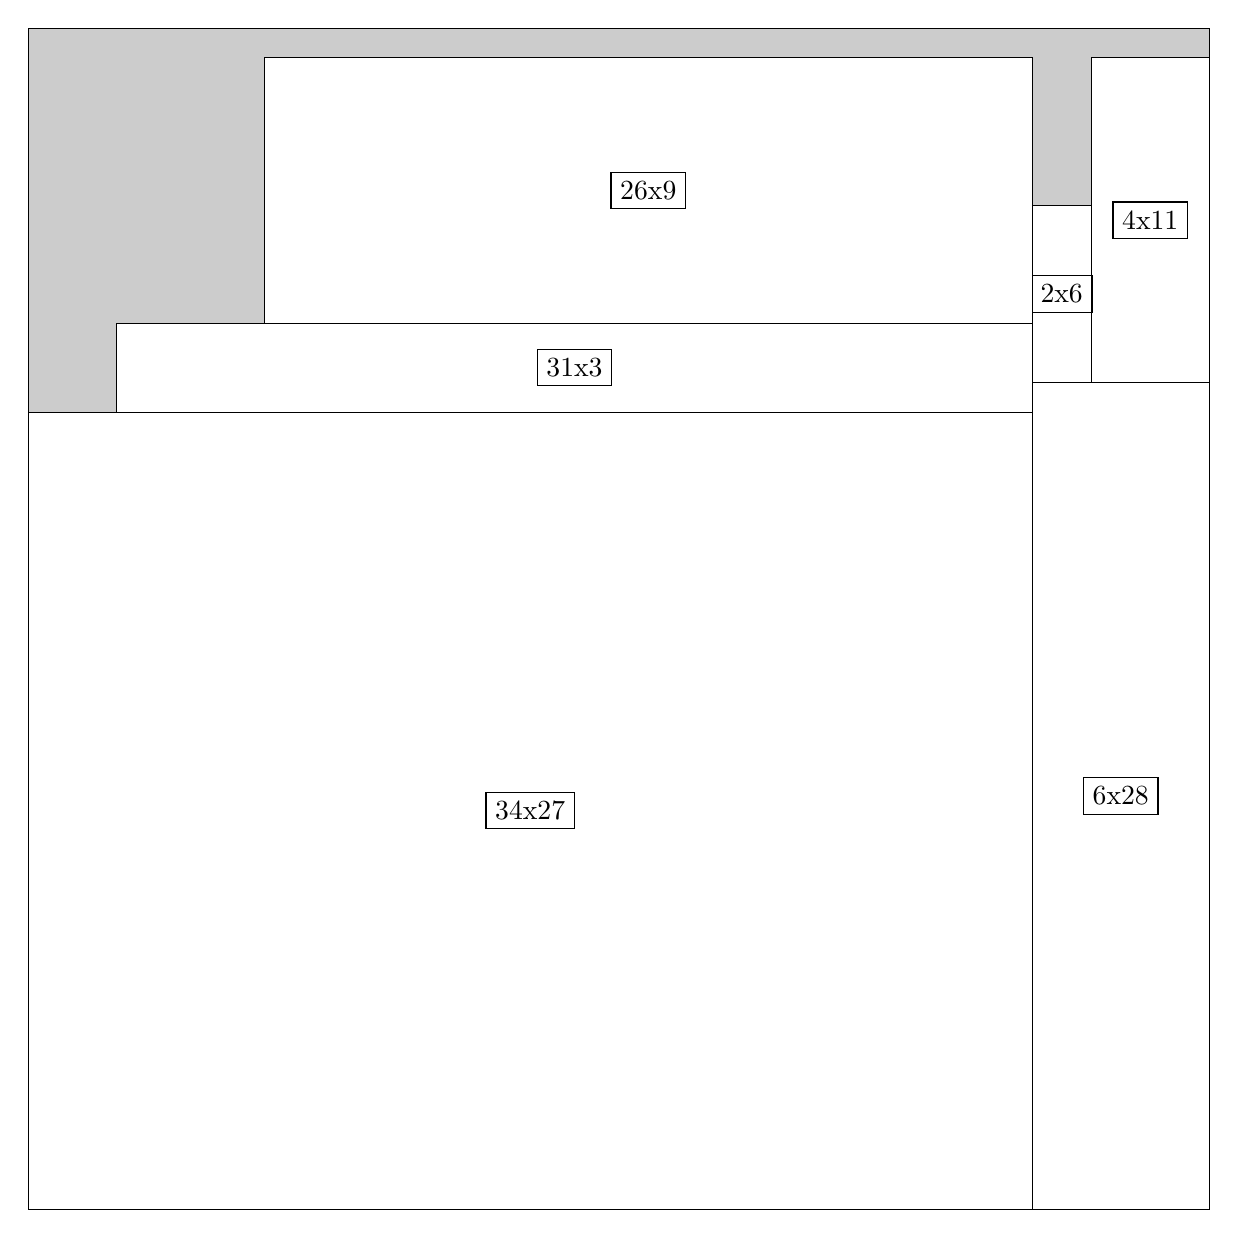
\begin{tikzpicture}[shorten >=1pt,scale=1.0,every node/.style={scale=1.0},->]
\tikzstyle{vertex}=[circle,fill=black!25,minimum size=14pt,inner sep=0pt]
\filldraw[fill=gray!40!white, draw=black] (0,0) rectangle (15.0,15.0);
\foreach \name/\x/\y/\w/\h in {6x28/12.75/0.0/2.25/10.5,4x11/13.5/10.5/1.5/4.125,2x6/12.75/10.5/0.75/2.25,34x27/0.0/0.0/12.75/10.125,31x3/1.125/10.125/11.625/1.125,26x9/3.0/11.25/9.75/3.375}
\filldraw[fill=white!40!white, draw=black] (\x,\y) rectangle node[draw] (\name) {\name} ++(\w,\h);
\end{tikzpicture}


w =6 , h =28 , x =34 , y =0 , v =168
\par
w =4 , h =11 , x =36 , y =28 , v =44
\par
w =2 , h =6 , x =34 , y =28 , v =12
\par
w =34 , h =27 , x =0 , y =0 , v =918
\par
w =31 , h =3 , x =3 , y =27 , v =93
\par
w =26 , h =9 , x =8 , y =30 , v =234
\par
\newpage


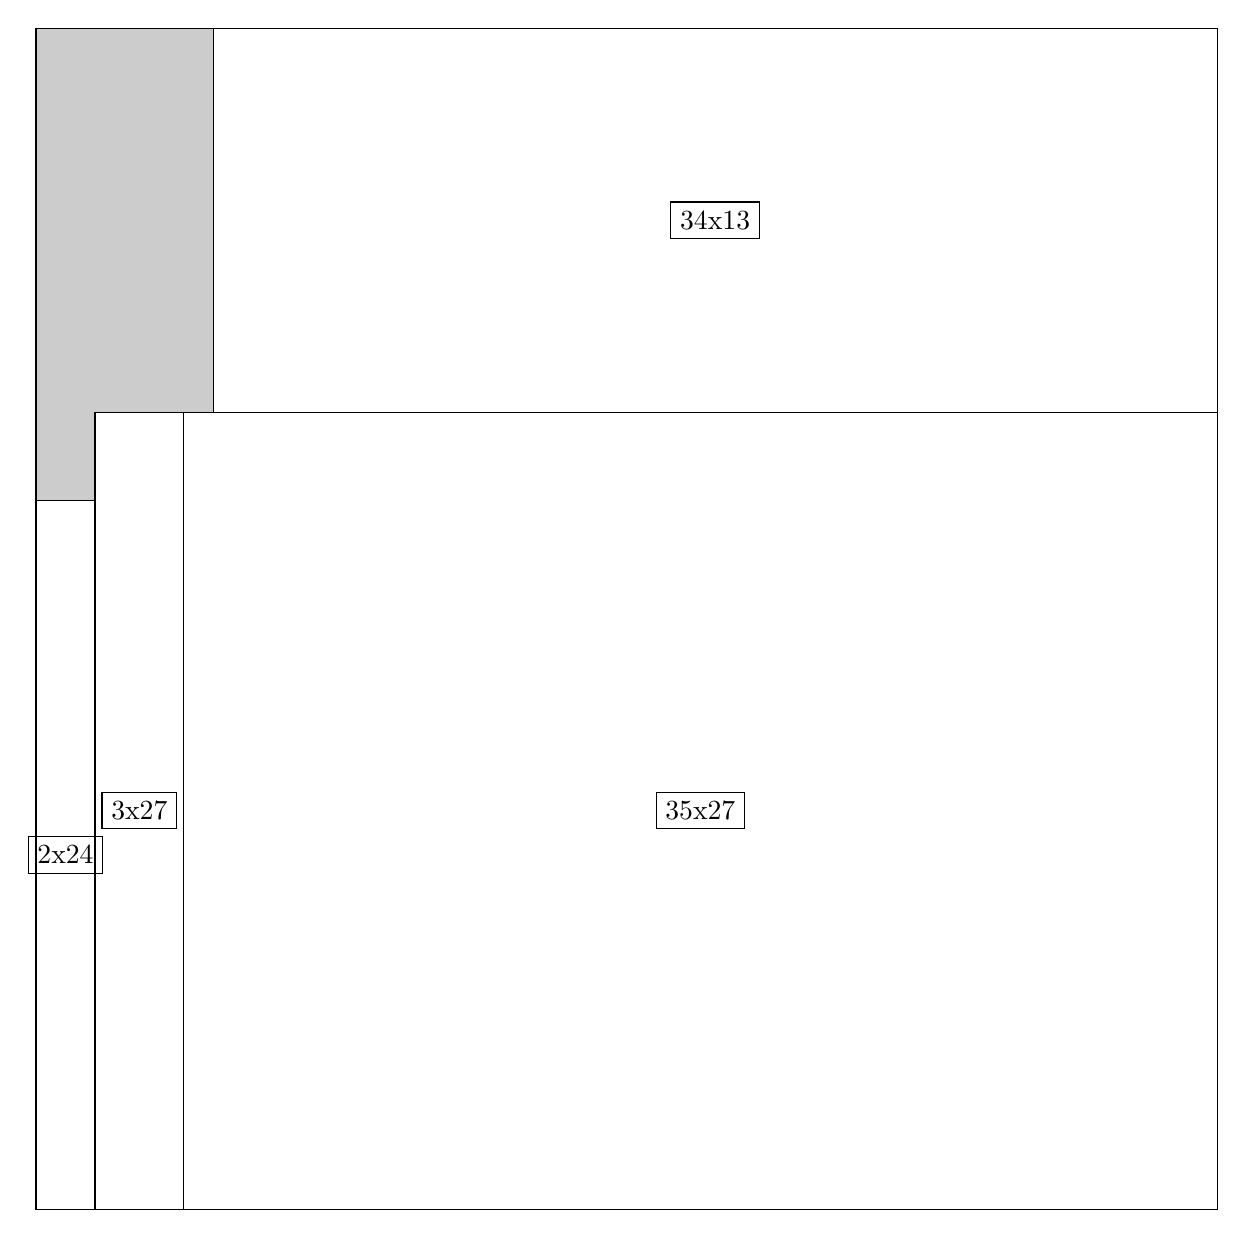
\begin{tikzpicture}[shorten >=1pt,scale=1.0,every node/.style={scale=1.0},->]
\tikzstyle{vertex}=[circle,fill=black!25,minimum size=14pt,inner sep=0pt]
\filldraw[fill=gray!40!white, draw=black] (0,0) rectangle (15.0,15.0);
\foreach \name/\x/\y/\w/\h in {35x27/1.875/0.0/13.125/10.125,3x27/0.75/0.0/1.125/10.125,2x24/0.0/0.0/0.75/9.0,34x13/2.25/10.125/12.75/4.875}
\filldraw[fill=white!40!white, draw=black] (\x,\y) rectangle node[draw] (\name) {\name} ++(\w,\h);
\end{tikzpicture}


w =35 , h =27 , x =5 , y =0 , v =945
\par
w =3 , h =27 , x =2 , y =0 , v =81
\par
w =2 , h =24 , x =0 , y =0 , v =48
\par
w =34 , h =13 , x =6 , y =27 , v =442
\par
\newpage


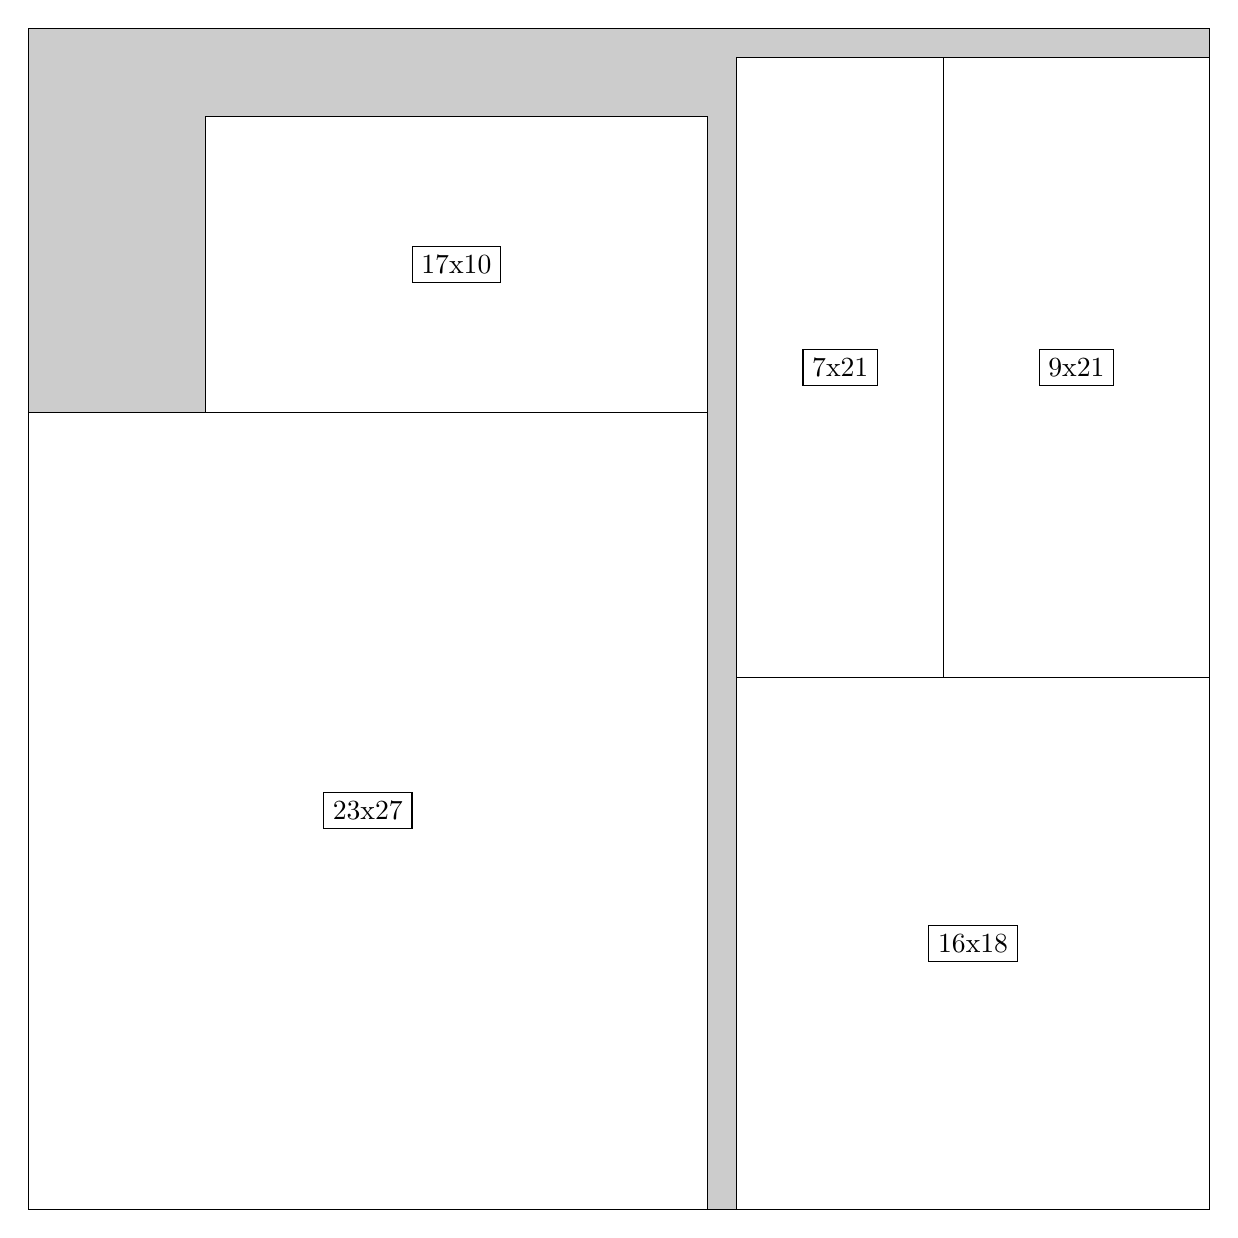
\begin{tikzpicture}[shorten >=1pt,scale=1.0,every node/.style={scale=1.0},->]
\tikzstyle{vertex}=[circle,fill=black!25,minimum size=14pt,inner sep=0pt]
\filldraw[fill=gray!40!white, draw=black] (0,0) rectangle (15.0,15.0);
\foreach \name/\x/\y/\w/\h in {16x18/9.0/0.0/6.0/6.75,9x21/11.625/6.75/3.375/7.875,7x21/9.0/6.75/2.625/7.875,23x27/0.0/0.0/8.625/10.125,17x10/2.25/10.125/6.375/3.75}
\filldraw[fill=white!40!white, draw=black] (\x,\y) rectangle node[draw] (\name) {\name} ++(\w,\h);
\end{tikzpicture}


w =16 , h =18 , x =24 , y =0 , v =288
\par
w =9 , h =21 , x =31 , y =18 , v =189
\par
w =7 , h =21 , x =24 , y =18 , v =147
\par
w =23 , h =27 , x =0 , y =0 , v =621
\par
w =17 , h =10 , x =6 , y =27 , v =170
\par
\newpage


\end{document}